%%%%%%%%%%%%%%%%%%%%%%%%%%%%%%%%%%%%%%%%%%%%%%%%%%%%%%%%%%%%%%%%%%%%%%%%%%%%%%%%%%%%%%%%%%%%%%%%%%%%%%%%%%%%%%%%%%%%%%%%%%%%%%%%%%%%%%%%%%
% 本文档基于复旦数院本科毕业论文标准模板定制
% 严格遵循 README 要求: 使用英文(半角)标点符号(除顿号、书名号外).
% 请使用xelatex对模板进行编译, 若想引用参考文献也能正确显示, 请依次按照xelatex->bibtex->xelatax->xelatex进行编译.
%%%%%%%%%%%%%%%%%%%%%%%%%%%%%%%%%%%%%%%%%%%%%%%%%%%%%%%%%%%%%%%%%%%%%%%%%%%%%%%%%%%%%%%%%%%%%%%%%%%%%%%%%%%%%%%%%%%%%%%%%%%%%%%%%%%%%%%%%%
\documentclass[a4paper,punct=banjiao,twoside]{ctexrep}

\usepackage[a4paper,hmargin={2.54cm,2.54cm},vmargin={3.175cm,3.175cm}]{geometry}
\headheight = 15 pt

\usepackage{amsmath,amssymb}
\usepackage{mathrsfs}

\usepackage[dvipsnames, svgnames, x11names]{xcolor}

\usepackage[colorlinks=true,linkcolor=Maroon]{hyperref}

\usepackage{amsthm}
% 配置定理环境
\theoremstyle{plain}
\newtheorem{thm}{定理}[chapter]
\newtheorem{lemma}[thm]{引理}
\newtheorem{axiom}[thm]{公理}
\newtheorem{coro}[thm]{推论}
\newtheorem{prop}[thm]{命题}
\newtheorem{con}[thm]{猜想}

\theoremstyle{definition}
\newtheorem{defn}[thm]{定义}
\newtheorem{asm}[thm]{假设}
\newtheorem{que}[thm]{问题}

\theoremstyle{remark}
\newtheorem{rem}{注}[chapter]
\newtheorem{example}{例}[chapter]

\renewcommand{\proofname}{\textbf{证明}}

\newcommand{\dd}{\text{d}}
\newcommand{\R}{{\mathbb R}}
\newcommand{\N}{{\mathbb N}}

% 其余的一些必要的宏包
\usepackage{xcolor,caption,array,enumerate}
\usepackage{graphicx} 
\usepackage{float} 
\usepackage{subcaption} 
\usepackage{tikz}

\usepackage{longtable, booktabs, threeparttable, caption, bicaption, multirow}
\usepackage[ruled,linesnumbered]{algorithm2e}

\usepackage{listings}
\lstset{
  language=Python, 
  basicstyle=\ttfamily, 
  breaklines=true, 
  keywordstyle=\bfseries\color{NavyBlue}, 
  morekeywords={}, 
  emph={self}, 
  emphstyle=\bfseries\color{Rhodamine}, 
  commentstyle=\itshape\color{black!50!white}, 
  stringstyle=\bfseries\color{PineGreen!90!black}, 
  columns=flexible,
  numbers=left, 
  numbersep=2em, 
  numberstyle=\footnotesize, 
  frame=single, 
  framesep=1em 
}

% 自定义多级标题格式
\CTEXsetup[nameformat={\huge \heiti},titleformat={\huge \heiti},beforeskip={0.0cm},afterskip={1.2cm}]{chapter}
\usepackage{titlesec}
\titleformat{\section}[block]{\Large\centering\heiti\bfseries}{\arabic{chapter}.\arabic{section}}{1em}{}[]
\titleformat{\subsection}[block]{\large \heiti\bfseries}{\arabic{chapter}.\arabic{section}.\arabic{subsection}}{1em}{}[]
\titleformat{\subsubsection}[block]{\normalsize\bfseries}{\arabic{subsection}-\alph{subsubsection}}{1em}{}[]
\titleformat{\paragraph}[block]{\small\bfseries}{[\arabic{paragraph}]}{1em}{}[]

\usepackage{gbt7714}

%%%%%%%%%%%%%%%%%%%%%%%%%%%%%%%%%%%%%%%%%%%%%%%%%%%%%%%%%%%%%%%%%%%%%%%%%%%%%%%%%%%%%%%%%%%%%%%%%%%%%%%%%%%%%%%%%%%%%%%%%%%%%%%%%%%%%%%%%%
\begin{document}

% 封面部分 (根据 template 注释保留, 需要时可取消注释并填写)
%\begin{titlepage}
%    {
%        \hfill 
%        \footnotesize
%    \begin{tabular}{cc}
%        \makebox[4em][s]{学校代码}:&\makebox[5em][l]{10246}\\
%        \makebox[4em][s]{学号}:&\makebox[5em][l]{??300180???}\\
%    \end{tabular}
%    }
%    \vspace*{1.5cm}
%    \begin{center}
%        \begin{figure}[H] 
%            \centering 
%            \includegraphics[width=0.46\textwidth]{figs/fudan-name.pdf} 
%        \end{figure}
%        \vspace*{1.5cm}
%        \makebox[16em][s]{\LARGE{本科毕业论文}}
%        \vspace*{3cm}
%        {\bfseries \Large 论文题目}
%        \vspace*{1cm}
%        {\bfseries  English Title}
%        \vspace*{3cm}
%        \fontsize{14pt}{\baselineskip}\selectfont
%        \begin{tabular}{cc}
%            \makebox[6em][s]{院系}:&\makebox[8em][c]{数学科学学院}\\[1ex]
%            \makebox[6em][s]{专业}:&\makebox[8em][c]{数学与应用数学}\\[1ex]
%            \makebox[6em][s]{姓名}:&\makebox[8em][c]{XXX}\\[1ex]
%            \makebox[6em][s]{指导老师}:&\makebox[8em][c]{XXX \ 教授}\\[1ex]
%            \makebox[6em][s]{完成日期}:&\makebox[8em][c]{\today}\\[1ex]
%        \end{tabular}     
%    \end{center}
%\end{titlepage}

\renewcommand{\thepage}{\roman{page}}

% 改写目录标题的格式
\renewcommand{\contentsname}{目\quad 录}
\tableofcontents
\setcounter{page}{1}

\chapter*{摘\quad 要}
\addcontentsline{toc}{chapter}{摘要}
\normalsize

在此处撰写中文摘要. 简明扼要地概括论文的研究背景、LoRA-BIRM 的核心架构、计算解耦带来的速度提升 (如 4 分钟对齐 22 分钟的优势)、隐式正则化理论发现以及最终的实验结论. 

\vspace{1em}
\noindent{\textbf{关键词:}} 大语言模型; 参数高效微调; 低秩适配(LoRA); 不变风险最小化(IRM); 贝叶斯变分推断; 分布外泛化

\chapter*{Abstract}
\addcontentsline{toc}{chapter}{Abstract}
\normalsize

This is my English abstract. Write the English translation of your abstract here.

\vspace{1em}
\noindent{\textbf{Keywords:}} Parameter-Efficient Fine-Tuning; Low-Rank Adaptation (LoRA); Invariant Risk Minimization (IRM); Bayesian Inference; Out-of-Distribution Generalization\\
\noindent{\textbf{CLC code:}} TP391

\clearpage
\mbox{}
\thispagestyle{empty}

\renewcommand{\thepage}{\arabic{page}}
\setcounter{page}{1}

%%%%%%%%%%%%%%%%%%%% 正文部分 %%%%%%%%%%%%%%%%%%%%

\chapter{引言}

\section{研究背景与意义}
\subsection{分布外泛化(OOD)与因果特征学习的兴起}
近年来, 深度神经网络在计算机视觉、自然语言处理等多个领域取得了突破性进展, 甚至在特定任务上超越了人类水平. 然而, 这些卓越的性能高度依赖于一个基础的统计学假设: 训练数据与测试数据满足独立同分布(Independent and Identically Distributed, I.I.D.)条件~\cite{shen2021towards}. 在实际的开放世界应用中, 由于数据采集的设备、时间、地理位置及背景环境的不断变迁, 测试数据的分布往往会发生不可预知的偏移(Distribution Shift). 当面对这种分布外(Out-of-Distribution, OOD)数据时, 传统深度学习模型的预测性能常常会出现断崖式的下降~\cite{hendrycks2019benchmarking}.

导致模型泛化能力退化的根本原因在于, 传统基于经验风险最小化(Empirical Risk Minimization, ERM)的训练范式倾向于以“贪婪”的方式最小化训练误差. 在这种机制下, 模型极易捕获数据中与标签高度共现, 但并无实质因果联系的“虚假关联(Spurious Correlations)”~\cite{geirhos2020shortcut}. 例如, 在图像分类任务中, 若训练集里的“牛”大多出现在绿草地上, 模型可能会捷径式地将“绿色背景”的纹理特征与“牛”的标签强绑定. 一旦在测试集中遇到“沙滩上的牛”, 模型便无法进行正确识别~\cite{beery2018recognition}. 这种依赖数据集特有统计偏差进行“捷径学习(Shortcut Learning)”的现象, 极大限制了人工智能在自动驾驶、医疗诊断等高风险领域的安全落地.

为了打破纯统计相关性的局限, 学术界开始将目光投向因果推断(Causal Inference), 由此促生了“因果特征学习(Causal Feature Learning)”这一新兴研究热点~\cite{scholkopf2021toward}. 因果学习的核心思想是引导模型摒弃环境中易变的虚假关联(如图像背景、颜色偏见), 转而挖掘跨环境保持绝对不变的真实“因果特征”(如物体的几何轮廓、语义逻辑等)~\cite{peters2017elements}.

在此背景下, Arjovsky 等人开创性地提出了不变风险最小化(Invariant Risk Minimization, IRM)框架~\cite{arjovsky2019invariant}. IRM 摒弃了将所有数据混合池化训练的传统方式, 转而引入了“环境(Environment)”的概念. 它假设无论数据的表层分布如何改变, 因果特征与标签之间的内在映射机制是恒定的. 因此, IRM 算法通过在目标函数中施加跨环境的损失方差或梯度一致性约束(Invariance Penalty), 强迫网络提取出在所有数据环境中均能适用同一个最优线性分类器的底层表征. 这一范式的提出, 为解决 OOD 泛化问题提供了一条极具潜力的数学路径, 并在此后迅速衍生出了包括方差外推风险最小化(V-REx)~\cite{krueger2021out} 以及本文所关注的贝叶斯不变风险最小化(BIRM)~\cite{lin2022bayesian} 等在内的一系列先进因果泛化算法, 成为了当前人工智能迈向“鲁棒通用智能”的核心基石.

\subsection{大规模神经网络在变分推断下面临的算力瓶颈}

近年来, 深度学习已经全面迈入大模型(Foundation Models)时代. 无论是计算机视觉领域的深层残差网络(ResNet)与视觉 Transformer(ViT), 还是自然语言处理领域的超大规模语言模型(LLM), 其参数量均呈现出指数级增长的趋势~\cite{kaplan2020scaling}. 尽管庞大的参数规模赋予了模型极其强大的特征拟合与泛化能力, 但这并未从根本上消除模型对数据中“虚假关联”的依赖. 因此, 将因果特征学习理论引入大规模预训练模型, 进而提升其在开放世界中的分布外泛化(OOD)能力, 成为了当前人工智能发展的必然方向.

然而, 理想的理论在向工程界迁移时, 往往会遭遇严酷的物理现实. 纵观当前因果泛化领域的最新文献, 绝大多数经典算法(包括传统的 IRM 以及贝叶斯变分推断版本)的实证研究, 依然高度局限于浅层多层感知机(MLP)或基础的微型卷积架构, 实验环境也多为结构简单的 Colored MNIST 等人工合成数据集~\cite{gulrajani2020search}. 

当研究者试图将这些复杂的因果约束(如跨环境的方差惩罚或梯度对齐)直接套用于现代深层网络时, 极易触发难以逾越的“算力墙(Compute Wall)”. 尤其是在引入贝叶斯变分推断来对抗“特征坍缩”时, 传统的全参数优化范式对算力和显存的需求超出了现有常规硬件的承受极限. 这种学术理论与工程规模之间的巨大“技术断层(Technical Gap)”, 使得大模型在面对复杂的分布偏移时依然缺乏有效的因果约束手段~\cite{wiles2021fine}. 

因此, 如何在千亿级参数的汪洋大海中, 以可接受的算力成本高效地寻找到那条绝对不变的“因果路径”, 使得深层神经网络能够真正受惠于贝叶斯因果理论, 构成了本课题研究的最核心宏观动机.

\section{现有因果学习算法的缺陷}
\subsection{全参数贝叶斯采样的巨大开销}
在因果学习的贝叶斯扩展方案中, 变分推断(Variational Inference, VI)是实现模型参数不确定性估计的核心机制~\cite{blundell2015weight}. 以贝叶斯不变风险最小化(BIRM)为例, 算法不再将神经网络的权重视为固定的点估计(Point Estimate), 而是假设其服从某种参数化的先验分布(如高斯分布). 在训练过程中, 模型通过优化证据下界(Evidence Lower Bound, ELBO), 不断逼近真实的后验分布~\cite{lin2022bayesian}. 这种机制虽然在对抗极端不变性惩罚(Invariance Penalty)时展现出了卓越的抗坍缩能力, 但其代价是引入了极其沉重的采样开销.

具体而言, 在全参数微调(Full-Parameter Fine-Tuning)范式下, 网络的前向传播(Forward Pass)必须依赖于重参数化技巧(Reparameterization Trick)来实现梯度的反向传播. 这意味着对于一个包含 $N$ 个参数的深度神经网络, 优化器不仅需要额外维护 $N$ 个方差参数, 还需要在每一次迭代时实时生成 $N$ 个高斯随机噪声变量. 当模型规模从简单的多层感知机(MLP)扩展到包含数千万甚至数十亿参数的现代架构(如 ResNet 或 Transformer)时, 这种逐参数(Parameter-wise)的随机采样操作会导致显存占用率瞬间飙升至原本的三倍以上~\cite{jospin2022hands}. 

更为严峻的是, 为了获得足够准确的期望梯度估计, 变分推断通常需要在单次参数更新中进行多次蒙特卡洛(Monte Carlo)前向采样. 这种成倍增加的计算负担, 使得全参数 BIRM 在处理高维图像或长文本数据时, 训练耗时呈指数级爆炸. 算力瓶颈已经成为了阻碍因果泛化算法从“玩具数据集(Toy Datasets)”走向工业级大模型的最主要物理屏障. 因此, 探索一种能够在大幅压缩采样维度的同时保留贝叶斯不确定性探索能力的新型架构, 成为了不可回避的工程挑战.

\subsection{高维参数空间下的优化坍缩与适配鸿沟}

除了前文所述的硬件算力爆炸, 传统的全参数不变风险最小化(IRM)及其贝叶斯扩展方案在向深层神经网络迁移时, 还面临着极其严峻的优化动力学(Optimization Dynamics)挑战. 

在浅层多层感知机(MLP)或微型卷积网络中, 模型的参数容量(Capacity)相对有限. 当算法在目标函数中施加强烈的不变性惩罚(Invariance Penalty)时, 模型依然能够在有限的特征空间内找到跨环境一致的因果特征. 然而, 当底座模型升级为包含千万级乃至百亿级参数的深度架构(如 ResNet 或 Transformer)时, 极高维的参数空间赋予了优化器过度的自由度(Degrees of Freedom)~\cite{lin2022bayesian}. 

在因果学习的博弈中, 预测损失(Predictive Loss)与环境方差惩罚往往存在剧烈的梯度冲突. 在极高的惩罚权重压迫下, 高维空间中的优化器为了以最快速度将环境间的损失方差“归零”, 往往会倾向于寻找一条投机取巧的捷径: 抹除所有学到的特征表示, 使得网络输出退化为平庸的常数或接近随机猜测的零解~\cite{geirhos2020shortcut}. 这种在高维过参数化(Over-parameterization)状态下极易触发的“梯度坍缩(Gradient Collapse)”现象, 导致全参数深层网络在因果泛化任务中表现出极不稳定的收敛轨迹, 经常在训练初期便陷入非预测性的退化解(Degenerate Solution). 

因此, 无论是从跨越“算力墙”的物理约束出发, 还是从抑制“高维特征坍缩”的数学需求出发, 传统的全参数微调范式都已陷入了死胡同. 破局的核心在于为因果约束过程引入一种“结构性瓶颈(Structural Bottleneck)”. 这促使我们将目光投向参数高效微调(PEFT)技术, 特别是低秩适配(LoRA)~\cite{hu2021lora}. 若能将沉重的贝叶斯变分推断下放至极低秩的适配器子空间中进行, 不仅有望从根本上消除计算灾难, 其低秩特性(Low-Rankness)更可以作为一种隐式正则化(Implicit Regularization)机制, 强制剥离高维空间中的虚假关联噪声. 这种将“因果惩罚”与“低秩结构”相融合的构想, 为打破当前的适配鸿沟提供了一条极具潜力的全新技术路径.

\section{主要研究内容与贡献}

针对传统贝叶斯不变风险最小化(BIRM)算法在深层神经网络中面临的算力瓶颈与高维优化坍缩问题, 本文创造性地将参数高效微调(PEFT)技术引入因果学习领域. 通过提出基于低秩结构的不变性学习架构, 本文致力于在“因果泛化能力”与“模型训练开销”之间寻找更优的平衡点. 具体而言, 本文的主要研究内容与核心贡献可归纳为以下三个方面: 

\subsection{参数高效因果学习架构的设计与实现}

本文首次提出了一种兼顾因果特征提取与极致算力优化的新型微调架构. 在该架构中, 庞大的预训练底座权重 $W_0 \in \mathbb{R}^{d \times k}$ 被完全冻结, 仅作为确定性的特征提取器; 而应对分布偏移的特征学习与贝叶斯推断, 则被约束在低秩适配器(LoRA)所构成的极小参数子空间内. 其前向传播的权重更新量被参数化为:
\begin{equation}
    \Delta W = B A, \quad \text{其中} \ A \in \mathbb{R}^{r \times k}, B \in \mathbb{R}^{d \times r}, \ r \ll \min(d, k).
\end{equation}
通过这种物理层面的“计算解耦”, 算法的总体优化目标演变为在低秩空间下寻找满足因果不变性的最优参数增量:
\begin{equation}
    \min_{A, B} \sum_{e \in \mathcal{E}_{tr}} \mathcal{L}^e(W_0 + BA) + \lambda \cdot \mathcal{R}_{inv}(W_0 + BA),
\end{equation}
其中 $\mathcal{L}^e$ 为环境 $e$ 下的经验风险, $\mathcal{R}_{inv}$ 为跨环境的一致性惩罚项. 这种设计从根本上规避了全参数高斯采样所引发的显存爆炸问题, 为大规模网络的因果微调提供了切实可行的路径.

\subsection{高维优化动力学分析与正则化机制}

在理论层面, 本文深入剖析了低秩参数空间在面对高压不变性惩罚时的优化动力学(Optimization Dynamics)特征. 研究发现, 在因果学习中, 极低秩的参数空间容量(Capacity Bottleneck)实际上扮演了隐式正则化(Implicit Regularization)的关键角色, 能够有效过滤高频的虚假关联噪声(Spurious Correlations). 

同时, 针对传统基于固定权重的高强度惩罚极易诱发模型“特征坍缩(Feature Collapse)”与“优化停滞”的退化现象, 本文提出并系统验证了平滑权重退火(Linear Weight Annealing)策略. 引入动态调节的惩罚强度 $\lambda(t)$, 能够缓解预测损失与方差惩罚之间的剧烈梯度冲突, 成功为低秩变分推断寻找到了平稳收敛的动力学边界.

\subsection{多尺度模型与分布偏移场景下的泛化验证}

在工程实证层面, 本文基于标准的分布外(OOD)泛化基准任务, 构建了高度受控的对比实验体系. 通过在不同规模的深层神经网络架构上进行测试, 验证了本文提出的低秩因果学习架构的普适性与鲁棒性. 

实验结果不仅定量展示了该架构在压缩单次迭代耗时、降低显存峰值等算力层面的显著优势, 更证明了模型在面临严重的训练集与测试集分布偏移时, 依然能够维持稳健的泛化精度. 这一验证不仅证明了低秩因果算法逻辑的完备性, 也为后续探索其在超大容量预训练模型(Foundation Models)以及更广泛的自然语言、计算机视觉下游任务中的迁移应用, 奠定了坚实的理论与工程基础.

\section{本文组织结构}

\chapter{预备知识与相关工作}

本章旨在为后续 LoRA-BIRM 的方法设计与理论分析建立统一的概念基础. 从全文的论证链条来看, 第 2 章的任务不是简单罗列文献, 而是回答三个前置问题: 第一, 为什么传统经验风险最小化在分布偏移下会失败, 以及 IRM/BIRM 试图修复的究竟是什么; 第二, 为什么参数高效微调中的低秩结构不仅是工程压缩技巧, 还可能成为因果学习中的结构性正则; 第三, 为什么一旦把贝叶斯推断与不变性约束同时带入大模型, 就会立刻遭遇高维优化与计算复杂度问题. 因此, 本章按照“因果泛化基础 $\rightarrow$ 低秩参数化基础 $\rightarrow$ 变分推断与优化基础”的顺序组织内容, 以便为第 3 章的 LoRA-BIRM 架构设计提供自然铺垫.

\section{因果泛化基础: 从 IRM 到 BIRM}

\subsection{IRM 的环境视角与基本目标}

不变风险最小化(Invariant Risk Minimization, IRM)是因果表征学习领域的奠基性框架~\cite{arjovsky2019invariant}. 传统的经验风险最小化(ERM)仅仅致力于最小化所有训练数据上的平均误差, 极易收敛于依赖数据集中特定统计偏差的“捷径解”. 为了提取跨域不变的因果特征, IRM 引入了“环境(Environment)”的概念, 将训练数据划分为多个来源于不同分布的子集. 

IRM 的核心假设是: 尽管不同环境中虚假特征与标签的关联强度可能剧烈波动, 但真实的因果特征与标签之间的映射关系在所有环境中必须保持绝对恒定. 基于此, IRM 在总体目标函数中引入了跨环境的一致性惩罚项(Invariance Penalty). 这种惩罚强制要求网络学习到一种数据表征, 使得在该表征之上构建的最优线性分类器能够在所有训练环境中同时达到最优(即各环境梯度的方差趋于零). 通过这种约束, IRM 理论上能够剥离环境中易变的虚假关联, 从而实现分布外(OOD)的鲁棒泛化.

\subsection{BIRM 的提出与坍缩修复}

尽管 IRM 在浅层模型上取得了显著成功, 但在面对更复杂的网络结构和更严苛的惩罚权重时, 往往会陷入“特征坍缩(Feature Collapse)”的困境. 当目标函数中的方差惩罚项权重极大时, 确定性的神经网络为了强行将各环境的差异降为零, 倾向于直接遗忘所有提取到的特征, 输出一个与输入无关的常数, 导致模型的预测能力完全丧失~\cite{lin2022bayesian}. 

为了克服这一优化陷阱, Lin 等人提出了贝叶斯不变风险最小化(Bayesian Invariant Risk Minimization, BIRM)~\cite{lin2022bayesian}. BIRM 摒弃了确定性的点估计, 引入变分推断(Variational Inference)将网络权重建模为概率分布. 通过在参数空间中注入不确定性噪声, BIRM 强迫模型在极高的惩罚压迫下依然保持对特征空间的探索能力, 从而在因果特征学习与预测准确率之间达成了更好的平衡. BIRM 的提出不仅极大提升了模型对抗坍缩的能力, 也确立了贝叶斯推断在因果泛化任务中的核心地位.

\subsection{SparseIRM 与结构性容量瓶颈的启发}

随着深度学习步入大模型时代, 研究者发现 IRM 框架在深层网络中存在一个内在的理论矛盾: 可训练性与泛化能力的对立~\cite{zhou2022sparse}. 现代神经网络通常需要过参数化(Overparameterization)来保证模型易于优化; 然而, Zhou 和 Lin 等人在后续研究中严谨地指出, 过参数化所引发的过拟合会轻易地摧毁 IRM 的不变性约束, 导致模型再次被高维的虚假特征所捕获~\cite{zhou2022sparse}. 

为了解决这一过参数化困境, 他们提出了稀疏不变风险最小化(Sparse Invariant Risk Minimization, SparseIRM)范式~\cite{zhou2022sparse}. SparseIRM 创造性地引入了全局稀疏约束(Global Sparsity Constraint), 通过限制模型在训练全过程中的特征选择预算(Feature Selection Budget), 使得模型无法在容量上“装下”高维的虚假关联噪声, 从而被强制要求选择低维且跨环境恒定的因果特征~\cite{zhou2022sparse}. 

SparseIRM 的成功深刻揭示了“结构性容量瓶颈”在因果学习中的关键正则化作用. 然而, 全局稀疏化通常需要在全量参数图上进行掩码(Mask)计算或复杂的结构剪枝操作, 难以直接且高效地迁移至拥有千亿参数的大语言模型(LLM). 这一理论发现直接启发了本文的核心动机: 既然“稀疏性(Sparsity)”能够作为因果特征的预算过滤器, 那么在数学空间上与其具备高度同构特性的“低秩性(Low-Rankness)”, 理应能够产生同等甚至更优的隐式正则化效果. 本文提出的 LoRA-BIRM 正是基于这一推论, 旨在以参数极度受限的低秩适配器替代全参数稀疏化, 以更低廉的计算成本打破大模型的过参数化困境.

\section{低秩参数化基础: 从 PEFT 到因果正则化}

\subsection{LoRA 的参数高效适配机制}

随着大语言模型(LLM)与超大规模视觉模型的参数量呈指数级攀升, 传统的全参数微调(Full-Parameter Fine-Tuning)在显存占用与计算开销上已逐渐触及硬件极限. 为此, 学术界提出了一系列参数高效微调(Parameter-Efficient Fine-Tuning, PEFT)技术, 旨在仅更新极少部分参数的前提下, 达到与全参数微调相媲美的下游任务性能. 其中, 低秩适配(Low-Rank Adaptation, LoRA)凭借其出色的训练效率与无推理延迟的优势, 成为了当前主流的微调范式~\cite{hu2021lora}.

LoRA 的核心思想基于一个重要的经验假设: 预训练模型在适配特定下游任务时, 其权重矩阵的内在更新量具有极低的本征维度(Intrinsic Dimension). 具体而言, 对于预训练模型中一个尺寸为 $d_{in} \times d_{out}$ 的冻结权重矩阵 $W_0$ , LoRA 通过旁路注入两个可训练的低秩矩阵 $A \in \mathbb{R}^{r \times d_{in}}$ 与 $B \in \mathbb{R}^{d_{out} \times r}$ 来近似表示权重的更新量 $\Delta W$ , 其中秩 $r \ll \min(d_{in}, d_{out})$ . 在前向传播过程中, 具有 LoRA 层的输出 $h$ 可表示为:
\begin{equation}
    h = W_0 x + \Delta W x = W_0 x + B A x.
\end{equation}

为了确保在微调起始阶段( $t=0$ )不破坏模型原有的预训练表征, LoRA 采用了一种非对称的初始化策略: 对降维矩阵 $A$ 采用随机高斯初始化, 而将升维矩阵 $B$ 严格初始化为零矩阵. 这保证了初始时刻 $\Delta W = BA = 0$ . 通过这种低秩分解, LoRA 能够将需要计算梯度的参数量压缩至原先的千分之一甚至更低, 极大地缓解了反向传播中的显存压力, 为将计算极其昂贵的变分推断(Variational Inference)引入大模型因果学习提供了物理上的可行性.

\subsection{低秩约束为何能够抑制虚假特征}

如前文所述, Zhou 等人提出的 SparseIRM 成功证明了“全局稀疏约束”可以通过限制特征选择预算来有效克服因果学习中的过参数化坍缩~\cite{zhou2022sparse}. 顺着这一理论脉络, 本文进一步指出: 稀疏性(Sparsity)与低秩性(Low-Rankness)在约束模型复杂度的拓扑流形上是高度同构的数学概念. 这种内在联系构成了本文利用 LoRA 替代 SparseIRM 进行因果约束的核心理论基石.

从矩阵分解与优化的视角来看, 稀疏性关注的是矩阵在标准正交基(即坐标轴)下非零元素的个数, 对应于 $L_0$ 或 $L_1$ 范数惩罚; 而低秩性则关注矩阵在奇异值空间中非零奇异值的个数, 对应于核范数(Nuclear Norm)惩罚或显式的低秩参数化. 换言之, “低秩”本质上就是“奇异值频谱上的稀疏”. 

在面对具有严重分布偏移的开放环境时, 虚假关联特征(如图像背景、高频纹理)通常张成了一个维度极高的非因果子空间 $\mathcal{Z}_{spu}$ ; 而真正的因果特征(如物体形状轮廓)则处于一个维度极低的因果子空间 $\mathcal{Z}_{inv}$ 中. 在全参数微调下, 权重矩阵拥有充裕的满秩自由度, 能够轻易在 $\mathcal{Z}_{spu}$ 中找到一条能够最小化经验风险的“捷径”, 从而导致泛化失败. SparseIRM 通过显式掩码(Mask)掐断了通向 $\mathcal{Z}_{spu}$ 的高维坐标连接; 而 LoRA 架构则通过将更新矩阵 $\Delta W$ 物理限制在极低的秩 $r$ 上, 使得模型从根本上缺乏足够的谱空间(Spectral Space)去拟合且记忆高维的虚假噪声.

当我们在目标函数中施加严酷的不变风险惩罚(IRM Penalty)时, LoRA 模型内部有限的低秩容量将面临极大的“预算挤压(Budget Squeeze)”. 为了在满足跨环境方差为零的前提下尽可能降低预测损失, 优化器将被迫放弃高维且在各环境间剧烈波动的虚假特征, 转而将低秩矩阵 $A$ 和 $B$ 的列空间严格对齐至低维且绝对稳定的因果子空间 $\mathcal{Z}_{inv}$ 上. 因此, 低秩空间在因果学习中天然充当了一个“隐式正则化器(Implicit Regularizer)”, 它以比全局稀疏化更低廉的计算成本、更友好的硬件兼容性, 实现了同等卓越的虚假特征过滤效果.

\section{变分推断与高维优化基础}

\subsection{ELBO 目标与重参数化技巧}

在因果学习的贝叶斯扩展中, 计算参数的真实后验分布 $P(W|\mathcal{D})$ 通常是不可解的(Intractable). 为此, 变分推断(Variational Inference, VI)引入了一个由参数 $\theta$ 控制的简单分布 $q_\theta(W)$ (如高斯分布)来逼近真实的后验分布. 这一逼近过程在数学上等价于最大化证据下界(Evidence Lower Bound, ELBO):
\begin{equation}
    \mathcal{L}_{ELBO} = \mathbb{E}_{W \sim q_\theta}[\log P(\mathcal{D}|W)] - \text{KL}(q_\theta(W) || P(W)).
\end{equation}
等式右侧的第一项为期望对数似然, 代表模型对数据的拟合与预测能力; 第二项为变分后验与先验分布之间的 KL 散度(Kullback-Leibler Divergence), 充当正则化项. 

为了允许梯度通过随机采样过程进行反向传播, Kingma 等人提出了著名的重参数化技巧(Reparameterization Trick)~\cite{kingma2013auto}. 该技巧将随机变量表示为确定性参数与无参数独立噪声的连续函数. 例如, 对于高斯分布 $q_\theta(W) = \mathcal{N}(\mu, \sigma^2)$ , 我们可以将其重参数化为:
\begin{equation}
    W = \mu + \sigma \odot \epsilon, \quad \text{其中} \ \epsilon \sim \mathcal{N}(0, I).
\end{equation}
通过这种变换, 损失函数关于均值 $\mu$ 与方差 $\sigma$ 的期望梯度的无偏估计得以高效计算. 然而, 正如本文在第 1 章中所指出的, 当网络参数维度 $d$ 极大时, 维持全量参数的均值与方差矩阵将带来极其庞大的显存开销, 且在每次迭代中生成 $d$ 维的高斯噪声也是巨大的计算瓶颈.

\subsection{高维因果优化的动力学困难}

在深层神经网络中, 极高的参数维度不仅放大了计算复杂度, 更深刻地改变了损失景观(Loss Landscape)的拓扑结构. 当目标函数中存在强烈的正则化惩罚(如 IRM 中的跨环境方差惩罚)时, 优化器在高维空间中面临着极其复杂的动力学博弈.

具体而言, 经验风险的下降梯度与环境方差惩罚的下降梯度在高维流形上往往呈现出近乎正交甚至完全相反的方向. 在过参数化(Overparameterization)状态下, 模型拥有无数个能够使得经验风险最小化的局部极小值(Local Minima). 然而, 面对极大的不变性惩罚权重 $\lambda$ , 优化器为了以最陡峭的方向降低惩罚项, 极易陷入病态的平庸解(Degenerate Solution)——即通过将所有特征权重 $\mu$ 衰减至接近于零, 从而换取方差惩罚项的绝对最小化(因为常数输出的方差恒为零).

这种“梯度坍缩(Gradient Collapse)”现象表明, 单纯依靠一阶优化算法很难在高维无约束空间中自发地寻找到既满足因果不变性、又保持极高预测能力的狭小“最优盆地(Optimal Basin)”. 本文引入的低秩(Low-Rank)约束, 不仅在物理层面上极大地削减了需要维护的变分参数数量, 更是通过改变损失景观的曲率(Curvature), 限制了模型走向平庸解的自由度. 这种将变分推断与低秩空间相融合的思路, 为突破高维因果优化的动力学困境提供了一条全新的理论通道.

\section{本章小结}

本章围绕 LoRA-BIRM 所依赖的三类基础知识完成了铺垫. 首先, 在因果泛化层面, 我们回顾了 IRM 如何通过环境不变性约束抵抗 shortcut, 以及 BIRM 与 SparseIRM 分别从贝叶斯不确定性和结构性容量限制两个方向修复 IRM 在深层网络中的失效. 其次, 在参数化层面, 我们说明了 LoRA 的低秩更新不仅是一种参数高效微调技术, 也能够在数学上充当虚假特征过滤器. 最后, 在优化层面, 我们指出高维变分推断与强不变性惩罚的结合会带来显著的复杂度与动力学难题. 这些分析共同导向同一个结论: 若要让因果约束真正迁移到大模型平台, 就必须同时在\textbf{参数空间}与\textbf{优化目标}两端引入结构性改造. 这正是下一章提出 LoRA-BIRM 架构的直接出发点.

\chapter{核心架构设计: LoRA-BIRM}

本章详细阐述 LoRA-BIRM 的完整架构设计. 该方法以低秩适配(LoRA)为变分推断的参数化载体, 将贝叶斯不变风险最小化(BIRM)的随机性约束在一个紧凑的低维子空间中实现, 从而在保留因果不变性学习能力的同时, 彻底规避了全参数变分推断在大规模语言模型上的计算灾难. 本章将依次介绍架构的计算解耦设计、优化动力学控制策略, 以及支撑实验的工具链实现细节.

\section{架构设计思路与计算解耦}

LoRA-BIRM 的核心设计哲学是\textbf{计算解耦}: 将预训练模型的确定性特征提取能力与因果不变性学习所需的随机性推断能力在物理层面上彻底分离. 这一解耦不仅是工程上的权宜之计, 更是对"哪些参数应当承载不确定性"这一深层问题的理论回答.

\subsection{确定性骨干提取与随机性低秩采样}

在标准的迁移学习范式中, 预训练语言模型的主干参数 $\mathbf{W}_0 \in \mathbb{R}^{d_{\text{out}} \times d_{\text{in}}}$ 被视为从海量语料中蒸馏出的通用语义知识, 其确定性是有保障的. 然而, 当模型需要在多个分布偏移的环境中学习因果不变特征时, 仅凭确定性的点估计参数无法对"哪些特征是真正因果的、哪些是虚假相关的"这一本质不确定性进行建模.

LoRA-BIRM 的解决方案是: \textbf{冻结骨干, 随机化低秩增量}. 具体而言, 对于预训练模型中的目标权重矩阵 $\mathbf{W}_0$, 其参数在整个训练过程中保持完全冻结, 仅通过一个低秩增量矩阵 $\Delta \mathbf{W}$ 进行任务适配:
\begin{equation}
    \mathbf{W} = \mathbf{W}_0 + \Delta \mathbf{W} = \mathbf{W}_0 + \mathbf{B} \mathbf{A},
\end{equation}
其中 $\mathbf{A} \in \mathbb{R}^{r \times d_{\text{in}}}$, $\mathbf{B} \in \mathbb{R}^{d_{\text{out}} \times r}$, 秩 $r \ll \min(d_{\text{out}}, d_{\text{in}})$. 在标准 LoRA 中, $\mathbf{A}$ 和 $\mathbf{B}$ 均为确定性参数. 而在 LoRA-BIRM 中, 我们对低秩矩阵 $\mathbf{A}$ 施加变分贝叶斯处理, 将其建模为一个矩阵高斯分布:
\begin{equation}
    \mathbf{A} \sim \mathcal{N}(\boldsymbol{\mu}_A, \text{diag}(\exp(\boldsymbol{\sigma}_A))),
\end{equation}
其中 $\boldsymbol{\mu}_A$ 和 $\boldsymbol{\sigma}_A$ 均为可学习的参数矩阵, 分别代表低秩适配方向的均值与对数方差. 在每次前向传播中, 通过重参数化技巧(Reparameterization Trick)对 $\mathbf{A}$ 进行独立采样:
\begin{equation}
    \mathbf{A} = \boldsymbol{\mu}_A + \boldsymbol{\epsilon} \odot \exp\!\left(\frac{1}{2}\boldsymbol{\sigma}_A\right), \quad \boldsymbol{\epsilon} \sim \mathcal{N}(\mathbf{0}, \mathbf{I}).
\end{equation}

这一设计的深刻之处在于: 骨干网络的确定性前向传播负责提取高质量的语义特征表示, 而低秩子空间中的随机采样则负责对因果特征的不确定性进行建模. 两者在计算图中相互独立, 互不干扰. 冻结骨干的另一个重要效果是\textbf{隐式正则化}: 低秩约束将变分参数的搜索空间从 $O(d_{\text{out}} \times d_{\text{in}})$ 压缩至 $O(r \times (d_{\text{out}} + d_{\text{in}}))$, 这一容量瓶颈(Capacity Bottleneck)从根本上限制了模型记忆虚假相关性的能力, 使其被迫在低维流形上寻找跨环境不变的特征方向.

此外, 由于变分参数的维度从数十亿降至数百万量级, KL 散度的计算从原本的维度灾难变为可以高效精确计算的封闭形式:
\begin{equation}
    D_{\text{KL}}\!\left(q(\mathbf{A}) \| p(\mathbf{A})\right) = \frac{1}{2} \sum_{i,j} \left( \exp(\sigma_{A,ij}) + \mu_{A,ij}^2 - 1 - \sigma_{A,ij} \right),
\end{equation}
其中先验 $p(\mathbf{A}) = \mathcal{N}(\mathbf{0}, \mathbf{I})$ 为标准高斯分布. 这一封闭形式的 KL 散度使得 ELBO 的优化无需蒙特卡洛近似, 大幅提升了训练的稳定性.

\subsection{联合损失函数重构与惩罚计算优化}

LoRA-BIRM 的训练目标是一个多项惩罚的联合损失函数, 其设计综合了 BIRM 的变分 ELBO 框架与 IRM 的跨环境不变性约束. 设训练数据来自 $K$ 个环境 $\{e_1, e_2, \ldots, e_K\}$, 每个环境的经验风险为 $\mathcal{R}^{e_k}(\theta)$, 则完整的训练目标为:
\begin{equation}
    \mathcal{L}_{\text{total}} = \underbrace{\frac{1}{K}\sum_{k=1}^{K} \mathcal{R}^{e_k}(\theta)}_{\text{NLL 项}} + \lambda(t) \cdot \underbrace{\left[\text{Var}_{k}\!\left(\mathcal{R}^{e_k}(\theta)\right) + \mathcal{P}_{\text{align}}\right]}_{\text{不变性惩罚项}} + \beta \cdot \underbrace{D_{\text{KL}}\!\left(q \| p\right)}_{\text{贝叶斯正则项}},
    \label{eq:lora_birm_loss}
\end{equation}
其中各项的含义如下:

\textbf{NLL 项}为所有环境上的平均负对数似然, 驱动模型在所有训练分布上保持基本的预测能力.

\textbf{不变性惩罚项}由两部分构成. 第一部分 $\text{Var}_{k}(\mathcal{R}^{e_k})$ 为跨环境损失方差, 直接惩罚不同环境间的风险差异, 迫使模型寻找在所有环境上均衡的特征表示. 第二部分 $\mathcal{P}_{\text{align}}$ 为对齐惩罚(Alignment Penalty), 用于度量同一批次内语义相似但环境标签不同的样本之间的预测一致性, 其计算方式为:
\begin{equation}
    \mathcal{P}_{\text{align}} = \frac{1}{2}\left(\left|\mathcal{R}^{e_1}_{\text{spu}} - \mathcal{R}^{e_1}_{\text{env}}\right| + \left|\mathcal{R}^{e_2}_{\text{spu}} - \mathcal{R}^{e_2}_{\text{env}}\right|\right),
\end{equation}
其中下标 $\text{spu}$ 和 $\text{env}$ 分别代表含有虚假相关性的样本子集与环境对照子集. 该项的引入使得模型不仅在宏观的环境级别上保持不变性, 还在微观的样本级别上对虚假特征的激活进行直接抑制.

\textbf{贝叶斯正则项} $D_{\text{KL}}(q \| p)$ 为变分后验与先验之间的 KL 散度, 其作用是防止低秩适配矩阵的方差参数 $\boldsymbol{\sigma}_A$ 退化为零(即退化为确定性的点估计), 从而维持模型对因果不确定性的持续建模能力. 超参数 $\beta$ 控制贝叶斯正则化的强度, 在实验中设置为 $\beta = 10^{-4}$.

在实现层面, 为了避免 KL 散度随模型隐层维度 $d_h$ 线性增长而导致的数值不稳定, 本文对 KL 项进行了维度归一化处理:
\begin{equation}
    \tilde{D}_{\text{KL}} = \frac{D_{\text{KL}}(q \| p)}{d_h},
\end{equation}
这一归一化确保了 KL 惩罚的量级在不同规模的模型上保持一致, 使得超参数 $\beta$ 具有跨模型的可迁移性.

\section{优化动力学控制: 平滑权重退火机制}

不变性惩罚权重 $\lambda(t)$ 的调度策略对 LoRA-BIRM 的训练稳定性具有决定性影响. 本节首先分析固定高惩罚权重导致的"休克疗法"缺陷, 随后介绍本文采用的线性动态退火策略.

\subsection{传统固定惩罚权重下的休克疗法缺陷}

在 IRM 及其早期变体的实现中, 不变性惩罚权重 $\lambda$ 通常被设置为一个固定的大常数(如 $\lambda = 100$ 或 $\lambda = 1000$). 这种"一步到位"的策略在理论上具有吸引力——更强的惩罚应当更快地迫使模型收敛至不变特征子空间. 然而, 在实践中, 这种"休克疗法"往往导致严重的\textbf{梯度坍缩(Gradient Collapse)}现象.

其根本原因在于优化初期的梯度竞争. 在训练开始阶段, 模型参数处于随机初始化状态, 不同环境的损失值差异极大, 导致方差惩罚项 $\text{Var}_k(\mathcal{R}^{e_k})$ 的梯度量级远超 NLL 项的梯度量级. 当 $\lambda$ 过大时, 优化器的更新方向几乎完全由惩罚项主导. 为了以最快速度降低跨环境方差, 最简单的策略是将所有特征权重压缩至零——因为常数预测的方差恒为零. 这一病态解(Degenerate Solution)在数学上满足不变性约束, 但在语义上毫无意义.

在贝叶斯框架下, 梯度坍缩还会引发额外的连锁反应: 当均值参数 $\boldsymbol{\mu}_A$ 被压缩至零时, KL 散度的梯度会进一步推动方差参数 $\boldsymbol{\sigma}_A$ 向先验收缩, 导致模型完全丧失对任务特征的适配能力. 这种"双重坍缩"在实验中表现为训练损失在极少数步骤内骤降至接近随机猜测水平, 且无法通过后续训练恢复.

\subsection{线性动态退火策略(Linear Annealing)的设计}

为克服上述缺陷, 本文设计了一种\textbf{线性动态退火(Linear Annealing)}策略, 其核心思想是: 在训练初期给予模型充分的"热身"时间, 让 NLL 项主导优化方向, 使模型首先建立起对任务的基本理解; 随后逐步引入不变性惩罚, 在已有特征表示的基础上温和地施加因果约束.

具体地, 惩罚权重 $\lambda(t)$ 按照如下分段线性函数随训练步数 $t$ 动态调整:
\begin{equation}
    \lambda(t) = \begin{cases}
        \lambda_{\text{peak}} \cdot \dfrac{t}{T_{\text{warm}}}, & t \leq T_{\text{warm}}, \\[6pt]
        \lambda_{\text{peak}}, & t > T_{\text{warm}},
    \end{cases}
    \label{eq:linear_annealing}
\end{equation}
其中 $\lambda_{\text{peak}}$ 为目标峰值惩罚权重, $T_{\text{warm}}$ 为预热步数. 在本文的实验设置中, $\lambda_{\text{peak}} = 10.0$, $T_{\text{warm}} = T_{\text{total}} / 3$, 即将总训练步数的前三分之一用于惩罚权重的线性爬升.

这一设计的理论依据来自于对损失景观的分析. 在预热阶段 $t \leq T_{\text{warm}}$, 较小的 $\lambda(t)$ 使得 NLL 梯度占主导, 模型在参数空间中首先找到一个具有合理预测能力的区域. 此时损失景观中的 NLL 极小值盆地(Basin)已经形成, 为后续的惩罚引入提供了稳定的"锚点". 在惩罚爬升阶段, 逐渐增大的 $\lambda(t)$ 温和地将优化轨迹从 NLL 极小值盆地引导至满足不变性约束的更优区域, 而不会因为惩罚梯度的突然主导而导致参数的剧烈震荡.

与余弦退火(Cosine Annealing)或指数退火等非线性调度相比, 线性退火具有两个显著优势: 其一, 惩罚增长速率恒定, 避免了非线性调度在某些阶段增长过快而在另一些阶段增长过慢的问题; 其二, 线性调度仅有两个超参数($\lambda_{\text{peak}}$ 和 $T_{\text{warm}}$), 调参成本极低, 且对超参数的敏感性较弱.

此外, 本文还引入了\textbf{指数移动平均(EMA, Exponential Moving Average)}机制作为训练稳定性的辅助保障. 在每个训练步骤结束后, 维护一个 EMA 模型参数 $\theta_{\text{ema}}$:
\begin{equation}
    \theta_{\text{ema}} \leftarrow \alpha \cdot \theta_{\text{ema}} + (1 - \alpha) \cdot \theta,
\end{equation}
其中衰减系数 $\alpha = 0.92$. EMA 模型通过对历史参数的加权平均, 有效平滑了训练过程中因惩罚权重变化引起的参数震荡, 使得模型在验证集上的性能曲线更加平稳. 在每个检查点(Checkpoint)处, 同时对当前模型和 EMA 模型进行完整的验证集评估, 并保留历史最优快照(Best Snapshot)作为最终模型, 以应对复杂场景下训练后期可能出现的性能回退问题.

\section{工具链与代码库建立}

为支撑上述架构设计的实验验证, 本文基于 PyTorch 和 HuggingFace PEFT 库构建了一套完整的 LoRA-BIRM 实验工具链. 本节介绍其中两个关键的工程实现细节.

\subsection{贝叶斯 LoRA 分类头的参数化构建}

LoRA-BIRM 的变分推断核心被封装在一个独立的 \texttt{BIRMLightweightHead} 模块中. 该模块接收预训练模型最后一层的隐层表示 $\mathbf{h} \in \mathbb{R}^{d_h}$ 作为输入, 并通过贝叶斯线性层输出分类 logits. 其参数化结构如下:

\begin{itemize}
    \item \textbf{均值参数} $\boldsymbol{\mu}_W \in \mathbb{R}^{C \times d_h}$: 分类权重矩阵的均值, 其中 $C$ 为类别数.
    \item \textbf{对数方差参数} $\boldsymbol{\sigma}_W \in \mathbb{R}^{C \times d_h}$: 分类权重矩阵的对数方差, 初始化为 $-3$ 以确保训练初期的方差较小, 避免过大的随机性干扰 NLL 的优化.
    \item \textbf{方差截断}: 为防止数值溢出, 对数方差被截断至区间 $[-8, 0]$, 对应方差范围 $[e^{-8}, 1]$.
\end{itemize}

在每次前向传播中, 通过重参数化技巧对权重矩阵进行独立采样:
\begin{equation}
    \mathbf{W} = \boldsymbol{\mu}_W + \boldsymbol{\epsilon} \odot \exp\!\left(\frac{1}{2} \text{clamp}(\boldsymbol{\sigma}_W, -8, 0)\right), \quad \boldsymbol{\epsilon} \sim \mathcal{N}(\mathbf{0}, \mathbf{I}).
\end{equation}

值得注意的是, 每次前向传播均进行\textbf{独立采样}, 而非在整个 mini-batch 内共享同一个噪声样本. 这一设计确保了不同样本的预测之间具有独立的随机性, 使得跨环境方差惩罚的估计更加准确, 避免了批内噪声相关性对惩罚梯度的污染.

在推断阶段, 为获得确定性的预测结果, 直接使用均值参数 $\boldsymbol{\mu}_W$ 进行前向传播, 不进行随机采样. 这一"均值推断"策略在理论上对应于变分后验的众数估计, 在实践中被证明比蒙特卡洛平均具有更低的方差和更高的计算效率.

\subsection{差分学习率与全量分批测试逻辑注入}

\textbf{差分学习率(Differential Learning Rate)}是 LoRA-BIRM 训练策略的重要组成部分. 由于贝叶斯分类头的参数从随机初始化开始训练, 而 LoRA 适配层的参数则在预训练权重的基础上进行微调, 两者所需的学习率量级存在显著差异. 本文采用如下差分学习率配置:

\begin{itemize}
    \item \textbf{贝叶斯分类头}: 学习率 $\eta_{\text{head}} = 3 \times 10^{-4}$, 较高的学习率使得分类头能够快速适应任务.
    \item \textbf{LoRA 适配层}: 学习率 $\eta_{\text{LoRA}} = 5 \times 10^{-5}$, 较低的学习率保护预训练知识不被过度覆盖.
\end{itemize}

两组参数通过 PyTorch 优化器的参数组(Parameter Group)机制分别配置, 共享同一个 AdamW 优化器实例, 以确保动量(Momentum)和自适应学习率的统计量在两组参数间独立维护.

\textbf{全量分批测试逻辑(Full-Batch Evaluation)}是保证模型选择可靠性的关键工程细节. 在早期实现中, 为节省验证时间, 每个检查点仅在验证集的随机子集(约 200 个样本)上进行评估. 然而, 这种近似评估引入了显著的噪声: 由于 LoRA-BIRM 的预测具有随机性(每次前向传播均进行独立采样), 小样本评估的准确率估计方差极大, 导致模型选择基于噪声信号而非真实性能. 在极端情况下, 一个在完整验证集上准确率仅为 51\% 的模型, 可能因为恰好在某个小批次上表现良好而被错误地选为最优快照.

为彻底消除这一问题, 本文在每个检查点处对\textbf{完整验证集}进行评估, 并在评估阶段切换至均值推断模式(关闭随机采样). 这一"全量确定性评估"策略确保了模型选择信号的可靠性, 是 LoRA-BIRM 在复杂 OOD 场景下取得稳定性能提升的重要工程保障.

为方便复现实验, 本文已将 CMNIST、Spurious CIFAR 与 Qwen 平台上的核心脚本、训练配置以及轻量结果摘要统一整理至 GitHub 仓库 \href{https://github.com/sunlay01/lora_birm}{https://github.com/sunlay01/lora\_birm}. 其中, Qwen 相关代码位于仓库的 \texttt{qwen/} 目录下, 包括 ERM、IRMv1、BIRM 与 LoRA-BIRM Snapshot 的主要训练脚本以及对应的结果汇总文件.

\chapter{理论分析: 低秩参数空间下的因果优化动力学}

本章旨在从数学层面严谨地剖析因果特征学习的理论演进过程. 我们首先回归不变风险最小化(IRM)的原始代数与拓扑框架, 随后揭示其在有限样本与过参数化网络中的失效机制, 并最终证明低秩适配(LoRA)如何完美弥补这一理论缺陷.

\section{不变风险最小化(IRM)的理论基石与局限}

Arjovsky 等人~\cite{arjovsky2019invariant} 提出 IRM 的核心贡献在于, 首次在数学上证明了: 只要环境间的虚假特征扰动足够丰富, 模型就能唯一地识别出真实的因果表征. 为此, 必须首先引入“线性一般位置”这一代数几何假设.

\subsection{线性一般位置假设与问题定义}

考虑一个线性结构方程模型(Linear SEM). 假设输入特征 $X \in \mathbb{R}^d$ 可分解为真实的因果特征 $X_{inv} \in \mathbb{R}^{d_{inv}}$ 与虚假特征 $X_{spu} \in \mathbb{R}^{d_s}$ (其中 $d = d_{inv} + d_s$). 
所有环境 $e \in \mathcal{E}_{all}$ 共享相同的因果机制: $Y = \gamma^\top X_{inv} + \epsilon^e$. 设 $\Sigma^e = \mathbb{E}^e[X X^\top] \in \mathbb{R}^{d \times d}$ 为环境 $e$ 中的特征协方差矩阵. 

\begin{defn}[线性一般位置 (Linear General Position)~\cite{arjovsky2019invariant}]
\label{def:general_position}
如果对于任意非零向量 $v \in \mathbb{R}^d$, 集合 $\{ \Sigma^e v \}_{e \in \mathcal{E}_{tr}}$ 能够张成(Span)一个维度至少为 $r$ 的线性子空间, 则称训练环境集合 $\mathcal{E}_{tr}$ 处于度数(Degree)为 $r$ 的线性一般位置.
\end{defn}

该定义的直观几何意义是: 不同环境的协方差矩阵不能在同一个非平凡的方向上发生“共线”式的退化, 这是保证虚假特征在不同环境中产生足够差异性的数学前提.

\subsection{线性因果表征的可识别性}

基于定义 \ref{def:general_position}, 原论文给出了核心的可识别性证明. 设表征矩阵为 $\Phi \in \mathbb{R}^{r \times d}$, 顶层线性分类器为 $w \in \mathbb{R}^{1 \times r}$. 

\begin{thm}[IRM 线性表征可识别性 (原论文 Theorem 9~\cite{arjovsky2019invariant})]
\label{thm:irm_thm9}
假设训练环境集合 $\mathcal{E}_{tr}$ 处于度数为 $r$ 的线性一般位置. 如果训练环境的数量满足 $|\mathcal{E}_{tr}| > d - d_{inv} + \frac{d_{inv}}{r}$, 那么对于任意满足不变性约束 $\nabla_{w|w=w^*} \mathcal{R}^e(w \Phi) = 0, \forall e \in \mathcal{E}_{tr}$ 的数据表征 $\Phi$, 必然存在一个可逆线性变换 $S$, 使得 $\Phi X = S X_{inv}$. 即 $\Phi$ 中对应于虚假特征的列向量必定全为 $\mathbf{0}$, 彻底屏蔽了虚假关联.
\end{thm}

\begin{proof}
在均方误差风险下, 环境 $e$ 中的约束 $\nabla_{w} \mathcal{R}^e(w \Phi) = 0$ 等价于正规方程(Normal Equation):
\begin{equation}
    \Phi \mathbb{E}^e[X X^\top] \Phi^\top (w^*)^\top - \Phi \mathbb{E}^e[X Y] = 0.
\end{equation}
代入真实的数据生成机制 $Y = X_{inv}^\top \gamma + \epsilon^e$. 我们构造增广因果向量 $\tilde{\gamma} = [\gamma^\top, \mathbf{0}^\top]^\top \in \mathbb{R}^d$ (其在虚假特征维度上全为 0), 使得 $Y = X^\top \tilde{\gamma} + \epsilon^e$. 
由于噪声 $\epsilon^e$ 独立于 $X$, 正规方程可化简为:
\begin{equation}
    \Phi \Sigma^e \Phi^\top (w^*)^\top - \Phi \Sigma^e \tilde{\gamma} = 0 \implies \Phi \Sigma^e (\Phi^\top (w^*)^\top - \tilde{\gamma}) = 0, \quad \forall e \in \mathcal{E}_{tr}.
\end{equation}

定义残差向量 $v = \Phi^\top (w^*)^\top - \tilde{\gamma} \in \mathbb{R}^d$. 上式表明, 对于所有训练环境 $e$, 向量 $\Sigma^e v$ 均落在表征矩阵 $\Phi$ 的零空间(Null Space)内.
采用反证法. 假设 $v \neq 0$. 根据环境处于度数为 $r$ 的线性一般位置, 向量组 $\{ \Sigma^e v \}_{e \in \mathcal{E}_{tr}}$ 至少张成了一个维度为 $r$ 的线性子空间. 
然而, 表征矩阵 $\Phi \in \mathbb{R}^{r \times d}$ 的最大秩为 $r$, 根据秩-零度定理(Rank-Nullity Theorem), $\Phi$ 的零空间维度最多为 $d - r$.
当环境数量 $|\mathcal{E}_{tr}|$ 满足定理中大于虚假特征秩的条件时, $\{ \Sigma^e v \}$ 张成的空间维度将超过 $\Phi$ 的零空间容量, 导致矛盾.
因此, 必定有 $v = \mathbf{0}$, 即 $\Phi^\top (w^*)^\top = \tilde{\gamma}$.
由于 $\tilde{\gamma}$ 在虚假特征对应的维度上严格为 $\mathbf{0}$, 且分类器 $w^*$ 为非零行向量, 这强制要求表征矩阵 $\Phi$ 在对应于 $X_{spu}$ 的列上必须全部为 $\mathbf{0}$. 证明完毕.
\end{proof}

\subsection{线性一般位置的测度论保证}

定理\ref{thm:irm_thm9}的结论极其强大, 但它高度依赖于“环境处于线性一般位置”这一代数前提. 为了证明该前提在现实数据中并不苛刻, 下面我们进一步给出了微分拓扑学(Differential Topology)与测度论上的兜底保证.

\begin{thm}[一般位置的测度论保证]
设 $\Sigma_{X,X}^e := \mathbb{E}_{X^e}[X^e (X^e)^\top] \in \mathbb{S}_{+}^{d \times d}$ (对称半正定矩阵空间). 对于任意固定的 $(\Sigma_{X,\epsilon}^e)_{e \in \mathcal{E}_{tr}}$, 使得训练环境集合 $\mathcal{E}_{tr}$ 不满足度数为 $r$ 的线性一般位置的协方差矩阵元组集合 $\{ (\Sigma_{X,X}^e)_{e \in \mathcal{E}_{tr}} \}$, 在空间 $(\mathbb{S}_{+}^{d \times d})^{|\mathcal{E}_{tr}|}$ 中的勒贝格测度为零(Lebesgue measure zero).
\end{thm}

\begin{proof}
令 $m = |\mathcal{E}_{tr}|$ 为环境数量. 定义映射 $G: \mathbb{R}^d \setminus \{0\} \rightarrow \mathbb{R}^{m \times d}$, 其元素为 $(G(x))_{e,i} = (\Sigma_{X,X}^e x - \Sigma_{X,\epsilon}^e)_i$.
令 $W = G(\mathbb{R}^d \setminus \{0\}) \subseteq \mathbb{R}^{m \times d}$. 这是一个维度至多为 $d$ 且缺失一个点的线性流形(Linear Manifold).

“不满足度数为 $r$ 的线性一般位置”, 等价于对于某些 $x \ne 0$, 矩阵 $G(x)$ 的秩小于或等于 $d-r$.
因此, 若令 $LR(m,d,k) \subseteq \mathbb{R}^{m \times d}$ 表示秩为 $k$ 的 $m \times d$ 矩阵的子流形, 我们需要证明: 当 $m > \frac{d}{r} + d - r$ 时, 对于一般的(generic) $(\Sigma_{X,X}^e)_{e \in \mathcal{E}_{tr}}$, 均有 $W \cap LR(m,d,k) = \emptyset$ (对于所有 $k < d-r$).

证明分为两步:
\textbf{第一步: 证明横截性 (Transversality).}
定义大映射 $F: (\mathbb{R}^d \setminus \{0\}) \times (\mathbb{S}_{+}^{d \times d})^m \rightarrow \mathbb{R}^{m \times d}$, 其中 $F(x, (\Sigma_{X,X}^e)_{e \in \mathcal{E}_{tr}})_l^{e'} = (\Sigma_{X,X}^{e'} x - \Sigma_{X,\epsilon}^{e'})_l$.
若能证明该映射的雅可比导数 $\nabla_{x,\Sigma_{X,X}} F$ 是满射(Surjective), 则 $F$ 必定横截于 $\mathbb{R}^{m \times d}$ 中的任意子流形(包括 $LR(m,d,k)$). 
根据 Thom 横截性定理(Thom's Transversality Theorem), 这将意味着使得 $W$ 与 $LR(m,d,k)$ 不横截相交的 $\Sigma_{X,X}^e$ 集合的测度为零.

要证 $\nabla_{x,\Sigma_{X,X}} F$ 是满射, 只需证 $\nabla_{\Sigma_{X,X}} F: (\mathbb{S}^{d \times d})^m \rightarrow \mathbb{R}^{m \times d}$ 是满射. 
计算偏导数 $\partial_{\Sigma_{i,j}^e} F_l^{e'} = \delta_{e,e'} (\delta_{l,i} x_j + \delta_{l,j} x_i)$.
对于任意目标矩阵 $C \in \mathbb{R}^{m \times d}$, 我们需要寻找对称矩阵组 $D \in (\mathbb{S}^{d \times d})^m$, 使得 $C_l^{e'} = \sum_{i,j,e} \delta_{e,e'} (\delta_{l,i} x_j + \delta_{l,j} x_i) D_{i,j}^e = (D^{e'} x)_l + (x D^{e'})_l$.
由于 $D^{e'}$ 是对称的, 这等价于 $C^{e'} = 2 D^{e'} x$. 
对于任意向量 $C^e$, 我们可以利用正交变换 $O$ 将 $x$ 旋转至非零基上, 并利用谱定理(Spectral Theorem)构造相应的特征值对角阵 $E^e$, 从而得到对称矩阵 $D^e = \frac{1}{2} O^\top E^e O$ 满足该方程. 
因此, 导数映射是满射, 横截性成立.

\textbf{第二步: 利用余维数(Codimension)计算排除相交.}
既然 $W$ 与 $LR(m,d,k)$ 几乎必然横截相交, 根据流形相交的维度定理, 它们的交集维度满足:
\begin{equation}
    dim(W \cap LR) = dim(W) + dim(LR(m,d,k)) - dim(\mathbb{R}^{m \times d}).
\end{equation}
根据代数几何常识, 秩为 $k$ 的矩阵流形其余维数 $codim(LR(m,d,k)) = (m-k)(d-k)$. 因此:
\begin{align}
    dim(W \cap LR) &= dim(W) - codim(LR(m,d,k)) \\
    &\le d - (m-k)(d-k).
\end{align}
当 $k < d-r$ 且环境数量 $m > \frac{d}{r} + d - r$ 时, 将这两个不等式代入上式:
\begin{align}
    dim(W \cap LR) &\le d - (m - (d-r))(d - (d-r)) \\
    &= d - r(m - d + r) \\
    &< d - r\left(\left(\frac{d}{r} + d - r\right) - d + r\right) \\
    &= d - d = 0.
\end{align}
交集的维度严格小于 $0$ 意味着交集必定为空集( $\emptyset$ ). 
因此, $W$ 中不存在秩小于 $d-r$ 的点, 从而环境集合几乎必然满足度数为 $r$ 的线性一般位置. 证明完毕.
\end{proof}

\subsection{理论的崩塌: 有限样本与过参数化的冲击}

Theorem 10 从数学上保证了在总体分布(Population Level)下失效概率几乎为零. 然而, Lin 等人(BIRM)~\cite{lin2022bayesian} 与 Zhou 等人(SparseIRM)~\cite{zhou2022sparse} 敏锐地指出, 这一优美的测度论保证在现代大模型微调中, 会遭遇“有限样本(Finite Samples)”与“过参数化(Overparameterization)”的双重夹击而彻底失效.

\begin{prop}[有限样本下全参数 IRM 的泛化失效~\cite{lin2022bayesian, zhou2022sparse}]
\label{prop:failure}
假设模型严重过参数化, 即参数总维度大于所有环境的有限样本量之和 ($d > \sum n_e$). 则必然存在一个完全依赖虚假与随机特征的过拟合权重矩阵 $W_{spu}$, 使得其在有限样本上的经验损失 $\hat{\mathcal{L}}(W_{spu})$ 恒等于 0, 从而完美绕过了 IRM 的总体测度限制.
\end{prop}

\begin{proof}
设 $n = \sum n_e$ 为有限的总样本量. 当模型过参数化时($d > n$), 经验数据上的线性方程组 $X W = Y$ 构成了一个典型的欠定系统(Underdetermined System). 
优化器可通过伪逆构造解 $W_{spu} = X^\top (X X^\top)^{-1} Y$, 仅利用高维虚假特征就完美插值(Interpolate)了所有有限训练样本.
此时在所有环境中均有经验风险 $\hat{\mathcal{R}}^e(W_{spu}) = 0$, 其经验梯度的方差自然恒为零. 
因此, 尽管 Theorem 10 保证了总体协方差不退化, 但在有限样本下, 极其高维的参数空间赋予了模型直接“作弊”的能力, 导致 IRM 约束在实践中形同虚设. 证明完毕.
\end{proof}
\section{贝叶斯扩展(BIRM)的理论与大模型的维度灾难}

如上一节所述, IRM 的理论保证在现实应用中常常失效. Lin 等人~\cite{lin2022bayesian} 在其提出的贝叶斯不变风险最小化(BIRM)理论中指出, 这一失效的根本原因在于深度模型的过拟合(Overfitting)倾向. 本节将严格重现其失效的数学证明, 介绍 BIRM 的变分解法, 并指出其在大语言模型(LLM)上遭遇的维度灾难.

\subsection{过参数化导致 IRM 坍缩的严格证明}

为了从代数上证明全参数 IRM 在过拟合时的退化现象, Lin 等人~\cite{lin2022bayesian} 提出了以下基础假设:

\begin{defn}[过拟合区域 (Overfitting Region)~\cite{lin2022bayesian}]
假设训练环境与样本数量有限(Assumption 1), 且特征提取器参数 $u$ 与分类器参数 $w$ 具有充足的容量来完全拟合训练数据(Assumption 2). 定义过拟合区域 $\Omega$ 为:
\begin{equation}
    \Omega := \{ (\bar{w}, \bar{u}) \mid \mathcal{R}^e(\bar{w}, \bar{u}) = 0, \forall e \in \mathcal{E}_{tr} \},
\end{equation}
其中 $\mathcal{R}^e$ 为定义在环境 $e$ 上的非负经验风险(Negative Log Likelihood).
\end{defn}

基于此, 原论文给出了 IRM 必然退化为经验风险最小化(ERM)的严格数学命题:

\begin{prop}[一般 IRM 的失效 (原论文 Proposition 1~\cite{lin2022bayesian})]
\label{prop:irm_failure}
在有限样本与充足容量的假设下, IRM 在区域 $\Omega$ 内退化为 ERM. 此外, $\Omega$ 中的任何元素都是一般 IRM 目标函数的合法解.
\end{prop}

\begin{proof}
一般 IRM 的优化目标要求解满足约束: $\bar{w} \in \arg\min_{w'} \mathcal{R}^e(w', \bar{u}), \forall e \in \mathcal{E}_{tr}$~\cite{lin2022bayesian}. 
对于任意过拟合解 $(\bar{w}, \bar{u}) \in \Omega$, 根据定义有 $\mathcal{R}^e(\bar{w}, \bar{u}) = 0$. 
由于模型被假设为良好设定的(Well-specified), 经验风险函数非负(即对于任意 $w, u$, 均有 $\mathcal{R}^e(w, u) \ge 0$)~\cite{lin2022bayesian}. 
因此, $0$ 是函数 $\mathcal{R}^e(w', \bar{u})$ 关于 $w'$ 的绝对全局极小值. 这意味着 $\bar{w}$ 必然是该最小化问题的一个最优解, 即严格满足了 IRM 的内在约束~\cite{lin2022bayesian}. 
此时, IRM 的惩罚项形同虚设, 模型完全退化为 ERM, 任何能够强行记忆数据的虚假特征都能“合法”地逃过不变性惩罚. 证明完毕.
\end{proof}

进一步地, 对于目前被广泛使用的 IRMv1 算法, 该坍缩现象同样成立:

\begin{thm}[IRMv1 的失效 (原论文 Corollary 1~\cite{lin2022bayesian})]
\label{thm:irmv1_failure}
假设 $\mathcal{R}^e(w,u)$ 关于参数可微, 那么对于任意 $(\bar{w}, \bar{u}) \in \Omega$, 如下等式成立:
\begin{equation}
    (\bar{w}, \bar{u}) \in \arg\min_{w,u} \sum_{e \in \mathcal{E}_{tr}} \mathcal{R}^e(w, u) + \lambda ||\nabla_{w} \mathcal{R}^e(w, u)||^2.
\end{equation}
\end{thm}

\begin{proof}
对于任意 $(\bar{w}, \bar{u}) \in \Omega$, 经验风险 $\mathcal{R}^e(\bar{w}, \bar{u}) = 0$. 由于 $0$ 是可微非负函数 $\mathcal{R}^e$ 的全局最小值, 根据微积分极值定理(Fermat's Interior Extremum Theorem), 该点处的第一变分(即梯度)必然为零: $\nabla_w \mathcal{R}^e(\bar{w}, \bar{u}) = 0$~\cite{lin2022bayesian}. 
将其代入 IRMv1 的目标函数中, 经验风险项为 $0$, 梯度惩罚项 $\lambda ||\mathbf{0}||^2 = 0$. 此时总体损失达到理论绝对下界 $0$. 优化器将不可避免地陷入这一包含虚假特征的平庸解中. 证明完毕.
\end{proof}

\subsection{BIRM 变分推断的引入}

为了打破确定性模型中“经验风险降为 0 则梯度必为 0”的死锁, Lin 等人提出 BIRM 框架, 放弃对分类器参数 $w$ 的点估计(Point Estimation), 转而利用变分推断(Variational Inference)学习参数的后验分布~\cite{lin2022bayesian}. 

设先验分布为 $p_0(w)$, 变分后验为 $q_u(w)$. 根据 BIRM 的推导, 后验分布的证据下界(ELBO)优化目标为~\cite{lin2022bayesian}:
\begin{equation}
    \max_{q_u} \sum_{e} \mathbb{E}_{q_u}[-\mathcal{R}^e(w,u)] - \text{KL}(q_u(w) || p_0(w)).
\end{equation}
通过强制要求后验分布 $q_u(w)$ 在所有环境下的行为保持一致(即引入跨环境的后验惩罚项), BIRM 在概率空间中实现了对虚假特征的有效过滤~\cite{lin2022bayesian}. 由于引入了 KL 散度(Kullback-Leibler Divergence)进行复杂度正则化, 使得模型无法坍缩为无限尖锐的 Dirac 冲激分布(即退化为点估计), 从而在理论上规避了 Proposition \ref{prop:irm_failure} 所指出的插值陷阱.

\subsection{大语言模型下 KL 散度的维度灾难}

尽管 BIRM 在中小型视觉模型上取得了显著成功~\cite{lin2022bayesian}, 但当我们将该变分框架直接迁移至参数量高达百亿级别( $d \sim 10^{10}$ )的大语言模型(LLM)时, 公式 (4.5) 中的变分正则项却引发了严重的“维度灾难”.

BIRM 默认采用平均场(Mean-Field)高斯近似来进行变分推断~\cite{lin2022bayesian}. 具体而言, 设模型参数总维度为 $d$, 先验分布设定为标准各向同性高斯 $p_0(w) = \mathcal{N}(\mathbf{0}, I_d)$, 变分后验设定为具有独立对角方差的高斯分布 $q_u(w) = \mathcal{N}(\mu, \text{diag}(\sigma^2))$. 

根据多元独立高斯分布的 Kullback-Leibler 散度解析式, 我们可以将 $\text{KL}(q_u || p_0)$ 分解为 $d$ 个独立维度的积分之和:
\begin{equation}
    \text{KL}(q_u || p_0) = \frac{1}{2} \sum_{i=1}^d \left( \mu_i^2 + \sigma_i^2 - \log \sigma_i^2 - 1 \right).
\end{equation}

在全参数微调(Full-Parameter Fine-Tuning)下, $d$ 是一个极其庞大的数字. 为了在下游任务中进行有效的确定性预测, 后验分布的方差 $\sigma_i^2$ 必须收缩(即 $\sigma_i^2 < 1$, 从而导致 $-\log \sigma_i^2 > 0$). 与此同时, 模型为了拟合有效特征, 其均值 $\mu_i$ 也会偏离初始值 $0$. 
即便每个独立维度上只产生了极微小的方差收缩或均值偏移, 这些微小的正数在经历 $d$ 次求和(即放大 $10^{10}$ 倍)后, 也会积聚成一个主导整个目标函数的巨大惩罚项. 因此, KL 散度的增长严格受控于 $\mathcal{O}(d)$.

这一代数推导揭示了一个残酷的优化动力学现实: 在大模型微调场景中, 参数量 $d$ 远远大于有限的训练样本量 $N$ (即 $d \gg N$). 此时, PAC-Bayesian 泛化界的复杂度惩罚项将正比于 $\mathcal{O}(\sqrt{d/N})$. 随着 $d \to \infty$, 泛化界将趋于无穷大, 彻底丧失了提供理论保证的意义.

更严重的是, 在实际的梯度优化过程中, 这种 $\mathcal{O}(d)$ 级别的 KL 散度项会呈现压倒性的绝对优势. 优化器为了避免产生巨大的惩罚, 会陷入“优化停滞(Optimization Stagnation)”——强行将所有参数的后验分布锁死在先验 $\mathcal{N}(\mathbf{0}, I_d)$ 附近(即强迫 $\mu \to 0, \sigma \to 1$), 导致经验风险 $-\mathcal{R}^e(w,u)$ 完全无法有效下降. 

因此, 想要在大语言模型中发挥 BIRM 的威力, 我们必须在数学空间上引入一种刚性的“降容”机制, 将变分推断的自由度从全参数的 $\mathcal{O}(d)$ 强行约束至一个极低的本征维度中.

\section{低秩参数空间下的隐式正则化与复杂度压缩}

前两节的分析表明, 现代大语言模型在进行因果表征学习时面临着“双重困境”: 一方面, 过参数化导致模型能够轻易通过插值绕过 IRM 的方差惩罚; 另一方面, 为解决插值问题而引入的 BIRM 变分推断, 又会因为大模型参数维度过高而导致 KL 散度爆炸, 引发优化停滞. 

本文提出的 LoRA-BIRM 架构, 放弃了在全参数空间中进行复杂的理论寻优, 转而将大模型的权重增量物理约束在极低秩的流形(Low-Rank Manifold)上. 本节将从参数自由度(Degrees of Freedom)与变分复杂度的角度, 阐明低秩架构如何自然地化解上述理论危机.

\subsection{容量挤压: 限制参数自由度打破插值陷阱}

全参数 IRM 失效的代数本质, 在于模型参数的自由度远远大于训练样本的约束数量. 在大语言模型的全参数微调中, 权重矩阵 $W \in \mathbb{R}^{d_{out} \times d_{in}}$ 拥有 $d_{out} \times d_{in}$ 个独立的自由度. 当这个量级远大于有限的样本量 $N$ 时, 经验风险优化的线性方程组处于极度的欠定状态(Underdetermined). 此时, 优化器完全有能力分配一部分冗余的参数维度, 去强行记忆(插值)各个环境中的高频虚假噪声, 从而使得经验风险和方差惩罚同时降为 0.

然而, 引入 LoRA 架构后, 这一代数前提被彻底打破. 预训练权重 $W_0$ 被冻结, 模型的有效优化空间被限制在旁路矩阵 $A \in \mathbb{R}^{r \times d_{in}}$ 和 $B \in \mathbb{R}^{d_{out} \times r}$ 中. 此时, 可学习参数的自由度锐减为:
\begin{equation}
    D_{LoRA} = r(d_{in} + d_{out}).
\end{equation}

由于秩 $r$ 通常被设定为极小的值(例如 4 或 8), $D_{LoRA}$ 远远小于全参数空间的自由度. 这种在物理结构上强制引入的“信息瓶颈(Information Bottleneck)”与“容量挤压(Capacity Squeeze)”, 带来了两个直接的正则化效果:
\begin{itemize}
    \item \textbf{方程适定性的转变}: 当 $D_{LoRA} < N$ 时, 优化问题从欠定系统转变为超定系统(Overdetermined System). 模型失去了在多环境中同时对虚假特征进行完美插值的代数能力. 经验风险 $\hat{\mathcal{R}}^e$ 无法被轻易“刷”到 0, 从而重新激活了 IRM 对跨环境梯度方差的惩罚机制.
    \item \textbf{隐式的特征选择}: 虚假特征(如背景、特定句式分布)通常具有高频且跨环境剧烈波动的特性. 极低秩的矩阵缺乏足够的基向量(Basis Vectors)去张成这些高维且复杂的虚假特征空间. 在优化过程中, 有限的秩预算(Rank Budget)会被迫优先分配给那些在所有环境中保持稳定、跨环境方差极小的低维因果特征. 
\end{itemize}

因此, 低秩约束在不需要引入额外复杂损失函数的前提下, 仅凭矩阵的代数性质就隐式地充当了一个“因果特征过滤器”.

\subsection{维度降维: 修复变分推断中的 KL 散度灾难}

在打破了插值陷阱后, 我们还需要确保 BIRM 的变分推断在大模型上能够正常收敛. 根据 4.2 节的推导, 全参数 BIRM 失效的根源在于: 对 $d_{out} \times d_{in}$ 规模的参数应用高斯变分后验时, 其偏离先验分布的 Kullback-Leibler (KL) 散度会呈现 $\mathcal{O}(d_{in} d_{out})$ 级别的爆炸, 导致总体目标函数被极大的惩罚项所吞噬.

在 LoRA-BIRM 架构中, 我们不再对庞大的全参数矩阵进行不确定性建模, 而是仅对低秩矩阵 $A$ 和 $B$ 赋予变分后验分布 $q_\theta(A, B)$. 
此时, 变分后验需要维护的独立分布参数(均值与方差)数量同样下降到了 $\mathcal{O}(r(d_{in} + d_{out}))$ 的量级. 

这种参数维度的断崖式下跌, 带来了统计学习理论上的关键修复:
\begin{equation}
    \text{KL}(q_\theta(A, B) || p_0(A, B)) \propto \mathcal{O}(r(d_{in} + d_{out})).
\end{equation}

将压缩后的 KL 散度代回至 BIRM 的泛化界框架中, 复杂度惩罚项从 $\mathcal{O}(\sqrt{d_{in}d_{out}/N})$ 骤降至 $\mathcal{O}(\sqrt{r(d_{in}+d_{out})/N})$. 只要微调数据量 $N$ 能够覆盖低秩参数的自由度, 该复杂度惩罚项就能收敛至一个合理且紧致(Tight)的数值区间内. 

在实际的梯度下降动力学中, 这意味着 KL 散度带来的正则化梯度, 终于能够与经验风险梯度、跨环境方差惩罚梯度处于同一个数值量级(Magnitude). 优化器不再会因为巨大的惩罚而陷入“锁死在先验”的停滞状态, 而是能够平稳地在低秩概率空间中探索, 找到既能拟合数据、又具备因果不变性、且不确定性适中的最优后验分布.

综上所述, LoRA 带来的“参数低秩化”不仅是工程上节省显存的妥协, 更是大模型因果表征学习中不可或缺的数学正则化器. 它从代数容量和统计复杂度两个层面, 完美修补了传统因果算法在过参数化网络中的理论漏洞.

\chapter{核心机理仿真与验证(基于 Colored MNIST)}

\section{任务定义、训练方法与评估协议}
\subsection{因果视觉任务定义: 引入虚假颜色的 CMNIST}
为了验证本文提出的低秩贝叶斯因果学习框架是否能够在最小可控场景下稳定工作, 本章首先选取 Colored MNIST (CMNIST) 作为核心机理验证平台. 选择该任务的原因在于: 其分布偏移由一个可解释、可精确操控的虚假特征所主导, 因而非常适合用于检验模型是否真正学到了跨环境不变的判别机制, 而不是继续依赖环境特有的统计捷径.

本文沿用经典二分类构造方式, 将原始 MNIST 数字按照“是否小于 5”映射为二元标签, 并进一步引入 $25\%$ 的标签扰动. 在此基础上, 每个样本被复制为两个颜色通道并仅保留其中一个通道, 从而使颜色成为显式的虚假特征. 训练阶段构造两个环境, 其颜色翻转概率分别设为 $e=0.2$ 与 $e=0.1$, 因而颜色与标签仍保持较强相关; 测试阶段构造一个更强的反转环境, 令 $e=0.9$, 即颜色与标签的相关方向几乎完全颠倒. 在这种设置下, 一个过度依赖颜色线索的模型将在训练环境中获得看似良好的经验风险, 但在测试环境中发生明显退化.

图~\ref{fig:cmnist_env_overview} 给出了本实验中三类环境的样本示意. 可以看到, 训练环境中的颜色偏置高度稳定, 而测试环境则刻意打破这种稳定性. 因此, 该任务本质上是在检验模型能否越过“颜色”这一捷径, 转而依赖数字形状这一跨环境不变特征.

\begin{figure}[htbp]
    \centering
    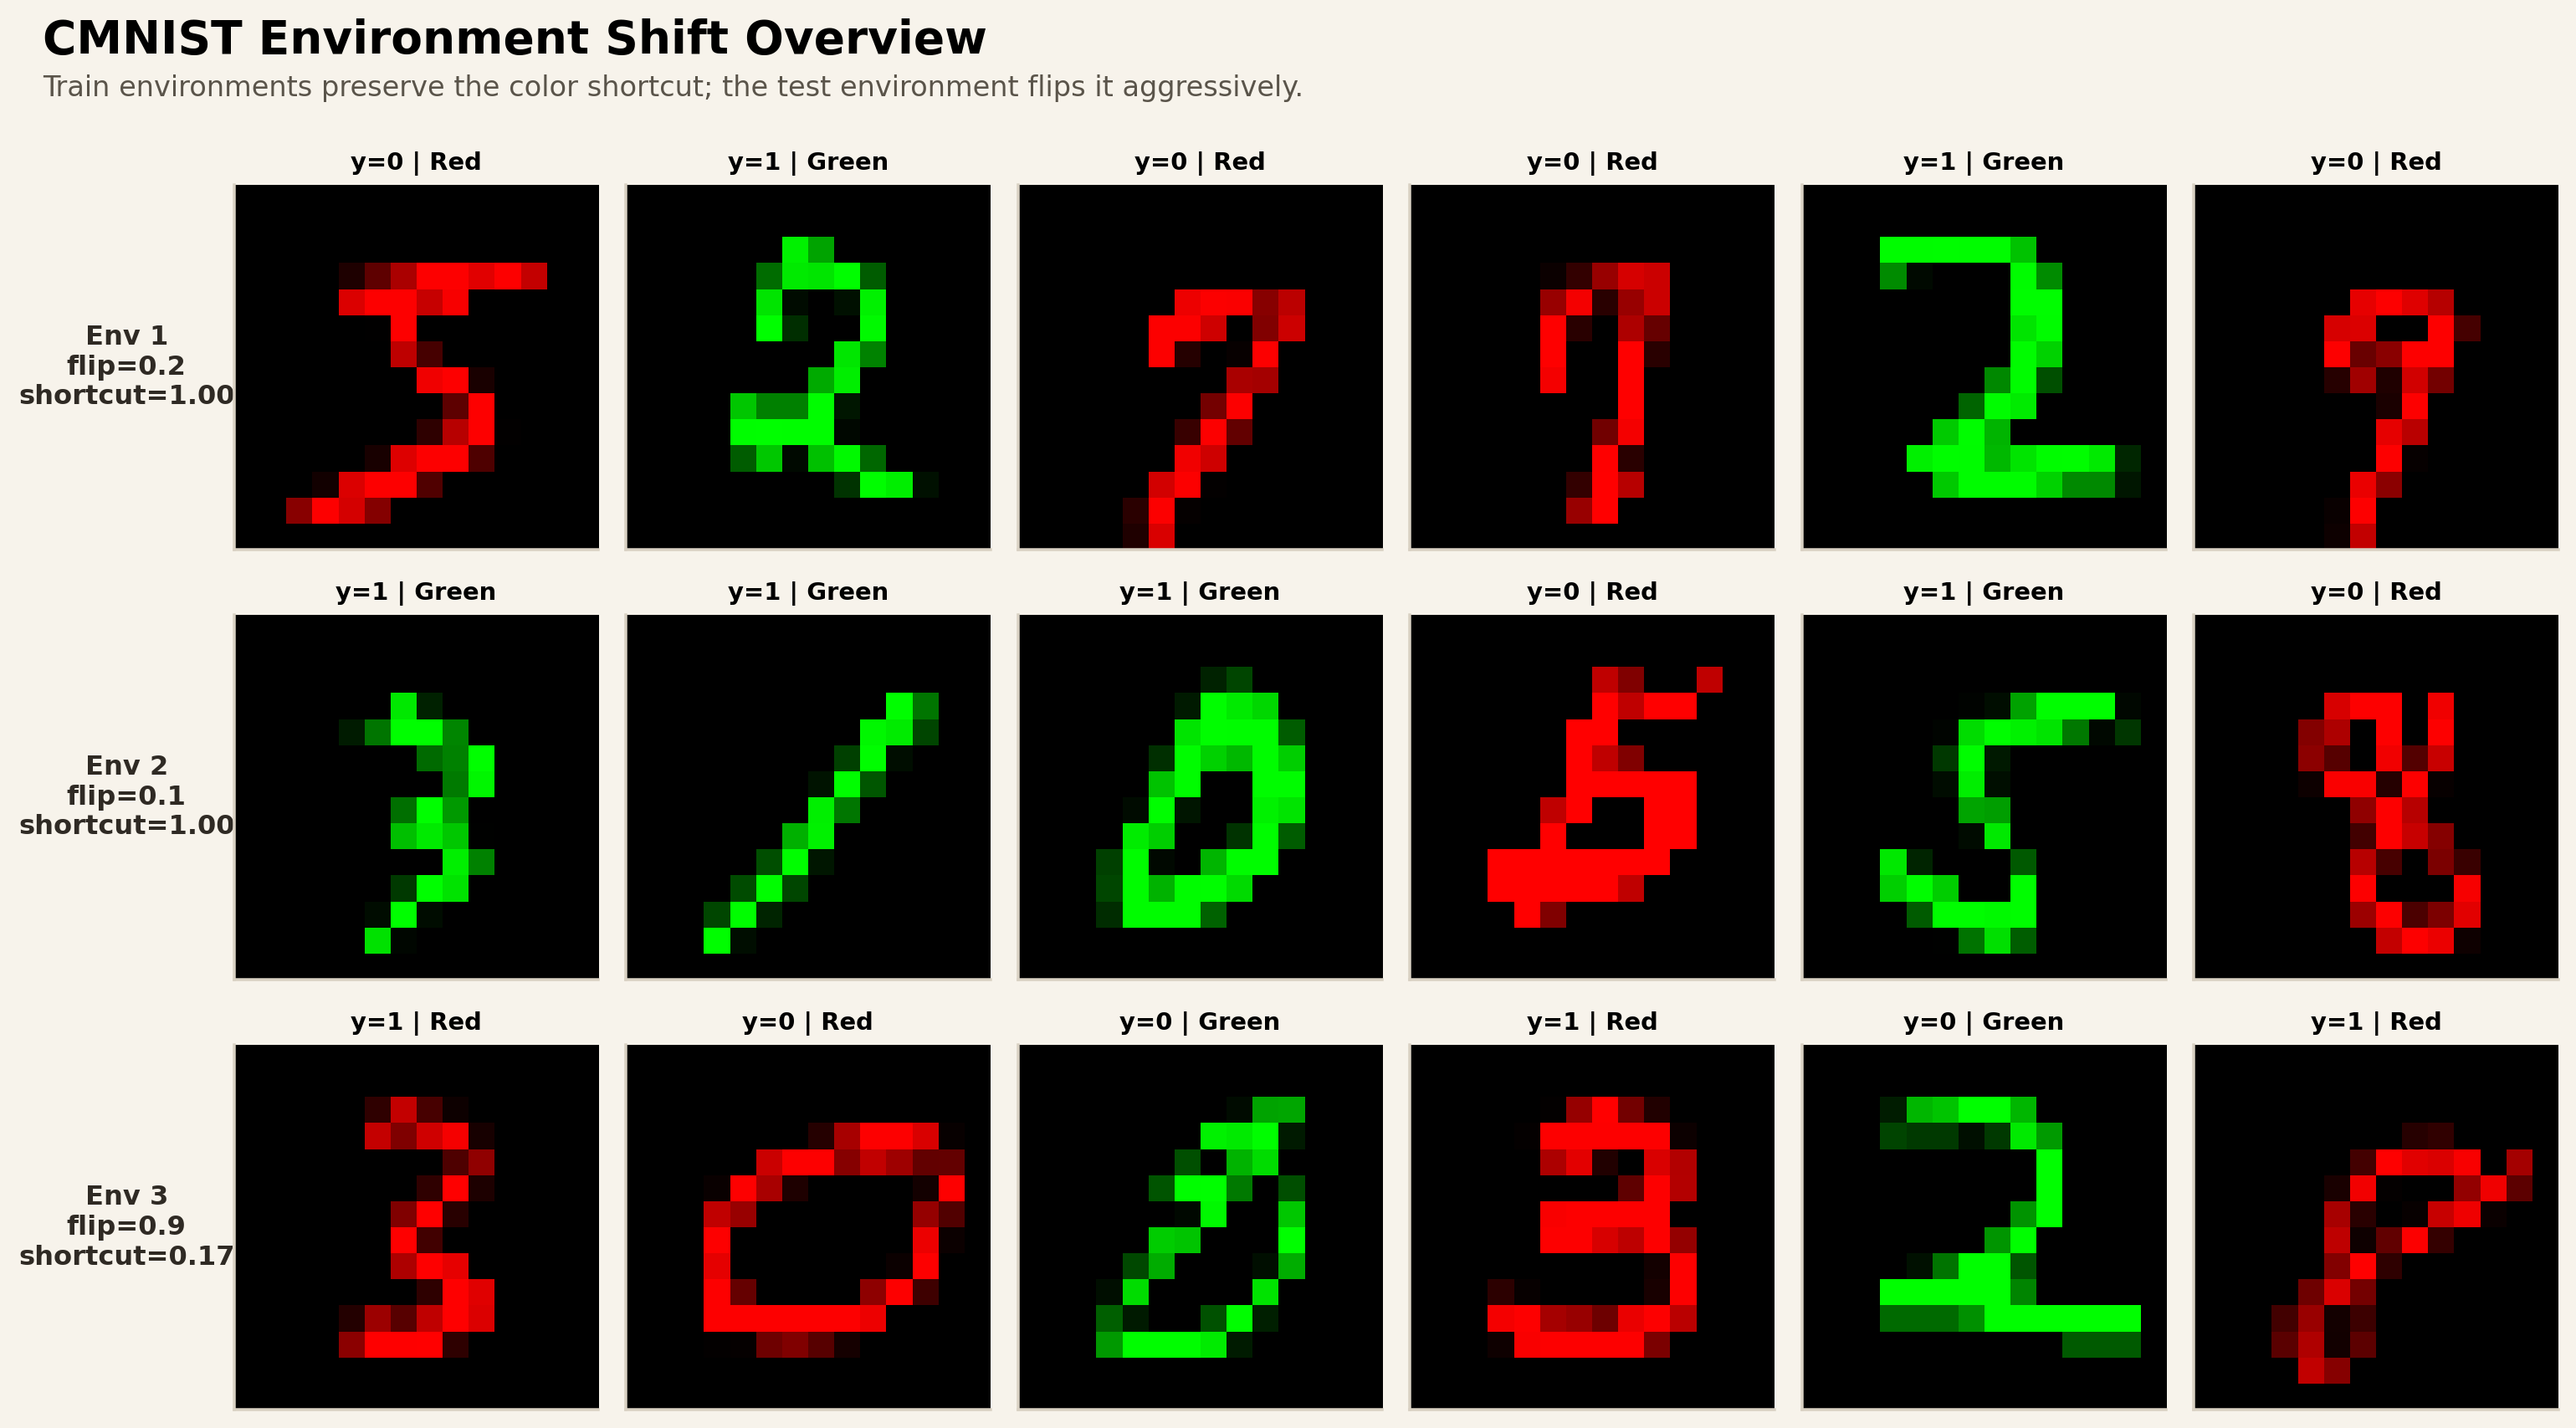
\includegraphics[width=\textwidth]{cmnist_environment_overview.png}
    \caption{CMNIST 三类环境的样本可视化. 前两个环境用于训练, 第三个环境用于分布外测试.}
    \label{fig:cmnist_env_overview}
\end{figure}

\subsection{四种方法的训练方式与评估协议}
为了尽可能公平地评估本文方法的有效性, 我们在同一份 CMNIST 数据划分上比较以下四类方法, 并统一使用训练环境外测试集上的 OOD 准确率作为核心指标:
\begin{itemize}
    \item \textbf{IRMv1}: 采用确定性多层感知机作为主干, 通过环境加权嵌入(EBD)计算 IRM 一阶梯度惩罚, 作为经典不变风险最小化基线.
    \item \textbf{Full-BIRM (Official)}: 保持与官方思路一致的全参数确定性骨干网络, 并在环境权重上施加蒙特卡洛采样后的贝叶斯不变性惩罚, 作为全参数 BIRM 基线.
    \item \textbf{LoRA-BIRM (Route A)}: 保持官方 EBD 惩罚逻辑不变, 仅将主干网络替换为确定性 LoRA 适配形式, 用于检验“低秩参数化”本身是否足以带来提升.
    \item \textbf{LoRA-BIRM (Route B)}: 采用真实的低秩变分推断路径, 在 LoRA 子空间中进行随机采样与环境方差惩罚, 是本文主张的核心实现路线.
\end{itemize}

四种方法虽然训练目标不同, 但训练协议保持一致: 都在相同的两环境 CMNIST 训练集上进行优化, 都以数字形状作为潜在因果特征、颜色作为显式虚假特征, 并在统一的反转测试环境上评估泛化能力. IRMv1 与 Full-BIRM 共享相同的全参数 MLP 主干; LoRA 两条路线则使用相同秩设置的低秩适配器, 区别只在于是否真正把贝叶斯随机性下放到低秩子空间中. 所有方法均独立运行 5 次, 每次训练 2000 步, 并记录测试环境上的最佳 OOD 准确率与总耗时. 这样的设计保证了本章比较的重点不在于网络容量大小的差异, 而在于\textbf{参数空间约束方式}与\textbf{不确定性建模方式}本身.

\section{结果一: OOD 泛化性能与方法排序}
\subsection{五次独立运行的 OOD 精度对比}
表~\ref{tab:cmnist_main_results} 汇报了 5 次独立运行后的平均 OOD 精度与运行时间. 从结果可以观察到三个核心现象.

第一, \textbf{LoRA-BIRM (Route B) 在 CMNIST 上取得了最优的平均 OOD 精度}. 其测试精度达到 $70.33 \pm 0.90\%$, 相较于 IRMv1 的 $68.71 \pm 1.43\%$ 提升了 $1.62$ 个百分点, 相较于 Full-BIRM 的 $68.96 \pm 0.90\%$ 也进一步提升了 $1.37$ 个百分点. 这一结果说明, 当贝叶斯不确定性被约束在低秩子空间中时, 模型并未因参数压缩而损失泛化能力, 反而在分布外环境中表现出更强的稳健性.

第二, \textbf{仅有低秩结构而没有真实的低秩变分推断, 并不足以稳定提升 OOD 泛化}. LoRA-BIRM (Route A) 的平均精度为 $68.24 \pm 1.49\%$, 不仅没有超过 Route B, 甚至略低于全参数基线. 这意味着低秩参数化虽然提供了结构瓶颈, 但若仍沿用确定性训练范式, 模型并不会自动获得更优的不变特征抽取能力. 真正产生增益的关键, 在于将\textbf{低秩结构约束}与\textbf{贝叶斯不确定性探索}联合起来.

第三, \textbf{Route B 在均值更高的同时保持了较低的方差}. 其标准差为 $0.90$, 与 Full-BIRM 持平, 但优于 IRMv1 和 Route A. 这表明本文方法并非偶然在个别随机种子下取得更优结果, 而是在重复实验中表现出更加稳定的收敛特征.

\begin{table}[htbp]
    \centering
    \caption{CMNIST 上 5 次独立运行的主结果.}
    \label{tab:cmnist_main_results}
    \begin{tabular}{lcc}
        \toprule
        方法 & 最佳 OOD 精度(\%) & 平均运行时间(s) \\
        \midrule
        IRMv1 & 68.71 $\pm$ 1.43 & 5.5 \\
        Full-BIRM (Official) & 68.96 $\pm$ 0.90 & 21.9 \\
        LoRA-BIRM (Route A) & 68.24 $\pm$ 1.49 & 23.7 \\
        LoRA-BIRM (Route B) & \textbf{70.33 $\pm$ 0.90} & 19.8 \\
        \bottomrule
    \end{tabular}
\end{table}

\subsection{低秩贝叶斯路线的理论可行性验证}
从理论视角看, 本章实验结果为第 4 章关于“低秩空间缓解高维因果优化困难”的分析提供了直接的经验支撑. Full-BIRM 虽然引入了不确定性建模, 但其优化仍在全参数空间附近展开, 因而在小样本、多环境冲突的设置下, 对稳定因果表征的提炼能力并不突出. 相比之下, Route B 将随机性显式压缩到 LoRA 子空间中, 使模型只能在一个更受限、更平滑的低维流形内完成环境对齐. 这类结构性约束实质上削弱了模型对高频虚假颜色模式的记忆能力, 并鼓励其优先保留跨环境共享的数字形状表征.

需要强调的是, CMNIST 毕竟属于低维玩具级任务. 因此, 本章的主要价值不在于单纯追求绝对分数的巨大领先, 而在于证明本文方法在最小可控平台上\textbf{能够工作、能够稳定工作, 且其收益方向与理论预期一致}. 对于一篇追求高水平学术质量的论文而言, 这一步是方法论成立的必要前提.

\section{结果二: 精度--效率折中关系}
\subsection{小规模平台上的训练代价比较}
从运行时间看, IRMv1 仍是本实验中最快的方法, 平均仅需 $5.5$s 即可完成单次训练. 这一本身并不令人意外, 因为 IRMv1 不涉及任何显式的贝叶斯采样或低秩随机推断. 然而, 若比较的是两类具备不确定性建模能力的方法, 则本文方法展现出了更具说服力的效率优势.

具体而言, Full-BIRM 的平均单次运行时间为 $21.9$s, 而 LoRA-BIRM (Route B) 为 $19.8$s, 在保持更高 OOD 精度的同时减少了约 $9.6\%$ 的训练耗时. 相比于 Route A 的 $23.7$s, Route B 也进一步减少了约 $16.5\%$ 的时间开销. 这说明在 CMNIST 这种小规模平台上, 低秩贝叶斯路线已经开始表现出“\textbf{精度更优且代价不升反降}”的趋势.

必须指出, 本章尚不足以完整体现本文所强调的“算力墙”优势. 原因在于 CMNIST 的输入分辨率、网络深度与样本复杂度都较低, 因而全参数 BIRM 的计算代价还未膨胀到不可接受的程度. 换言之, 本章结果更像是一次\textbf{趋势验证}, 而不是最终的工程极限展示.

\subsection{精度与稳定性的联合观察}
图~\ref{fig:cmnist_dashboard} 汇总展示了本章实验中的精度均值、时间均值、精度--效率散点关系以及多次运行稳定性. 从中可以更清楚地看到, Route B 位于右上方的更优区域: 它在 OOD 精度上领先于所有基线, 同时其运行时间又明显低于全参数 Full-BIRM. 这意味着本文方法并不是依靠简单地增加训练预算来“换取”精度, 而是在\textbf{参数空间设计}与\textbf{不确定性注入方式}两方面同时实现了更优平衡.

\begin{figure}[htbp]
    \centering
    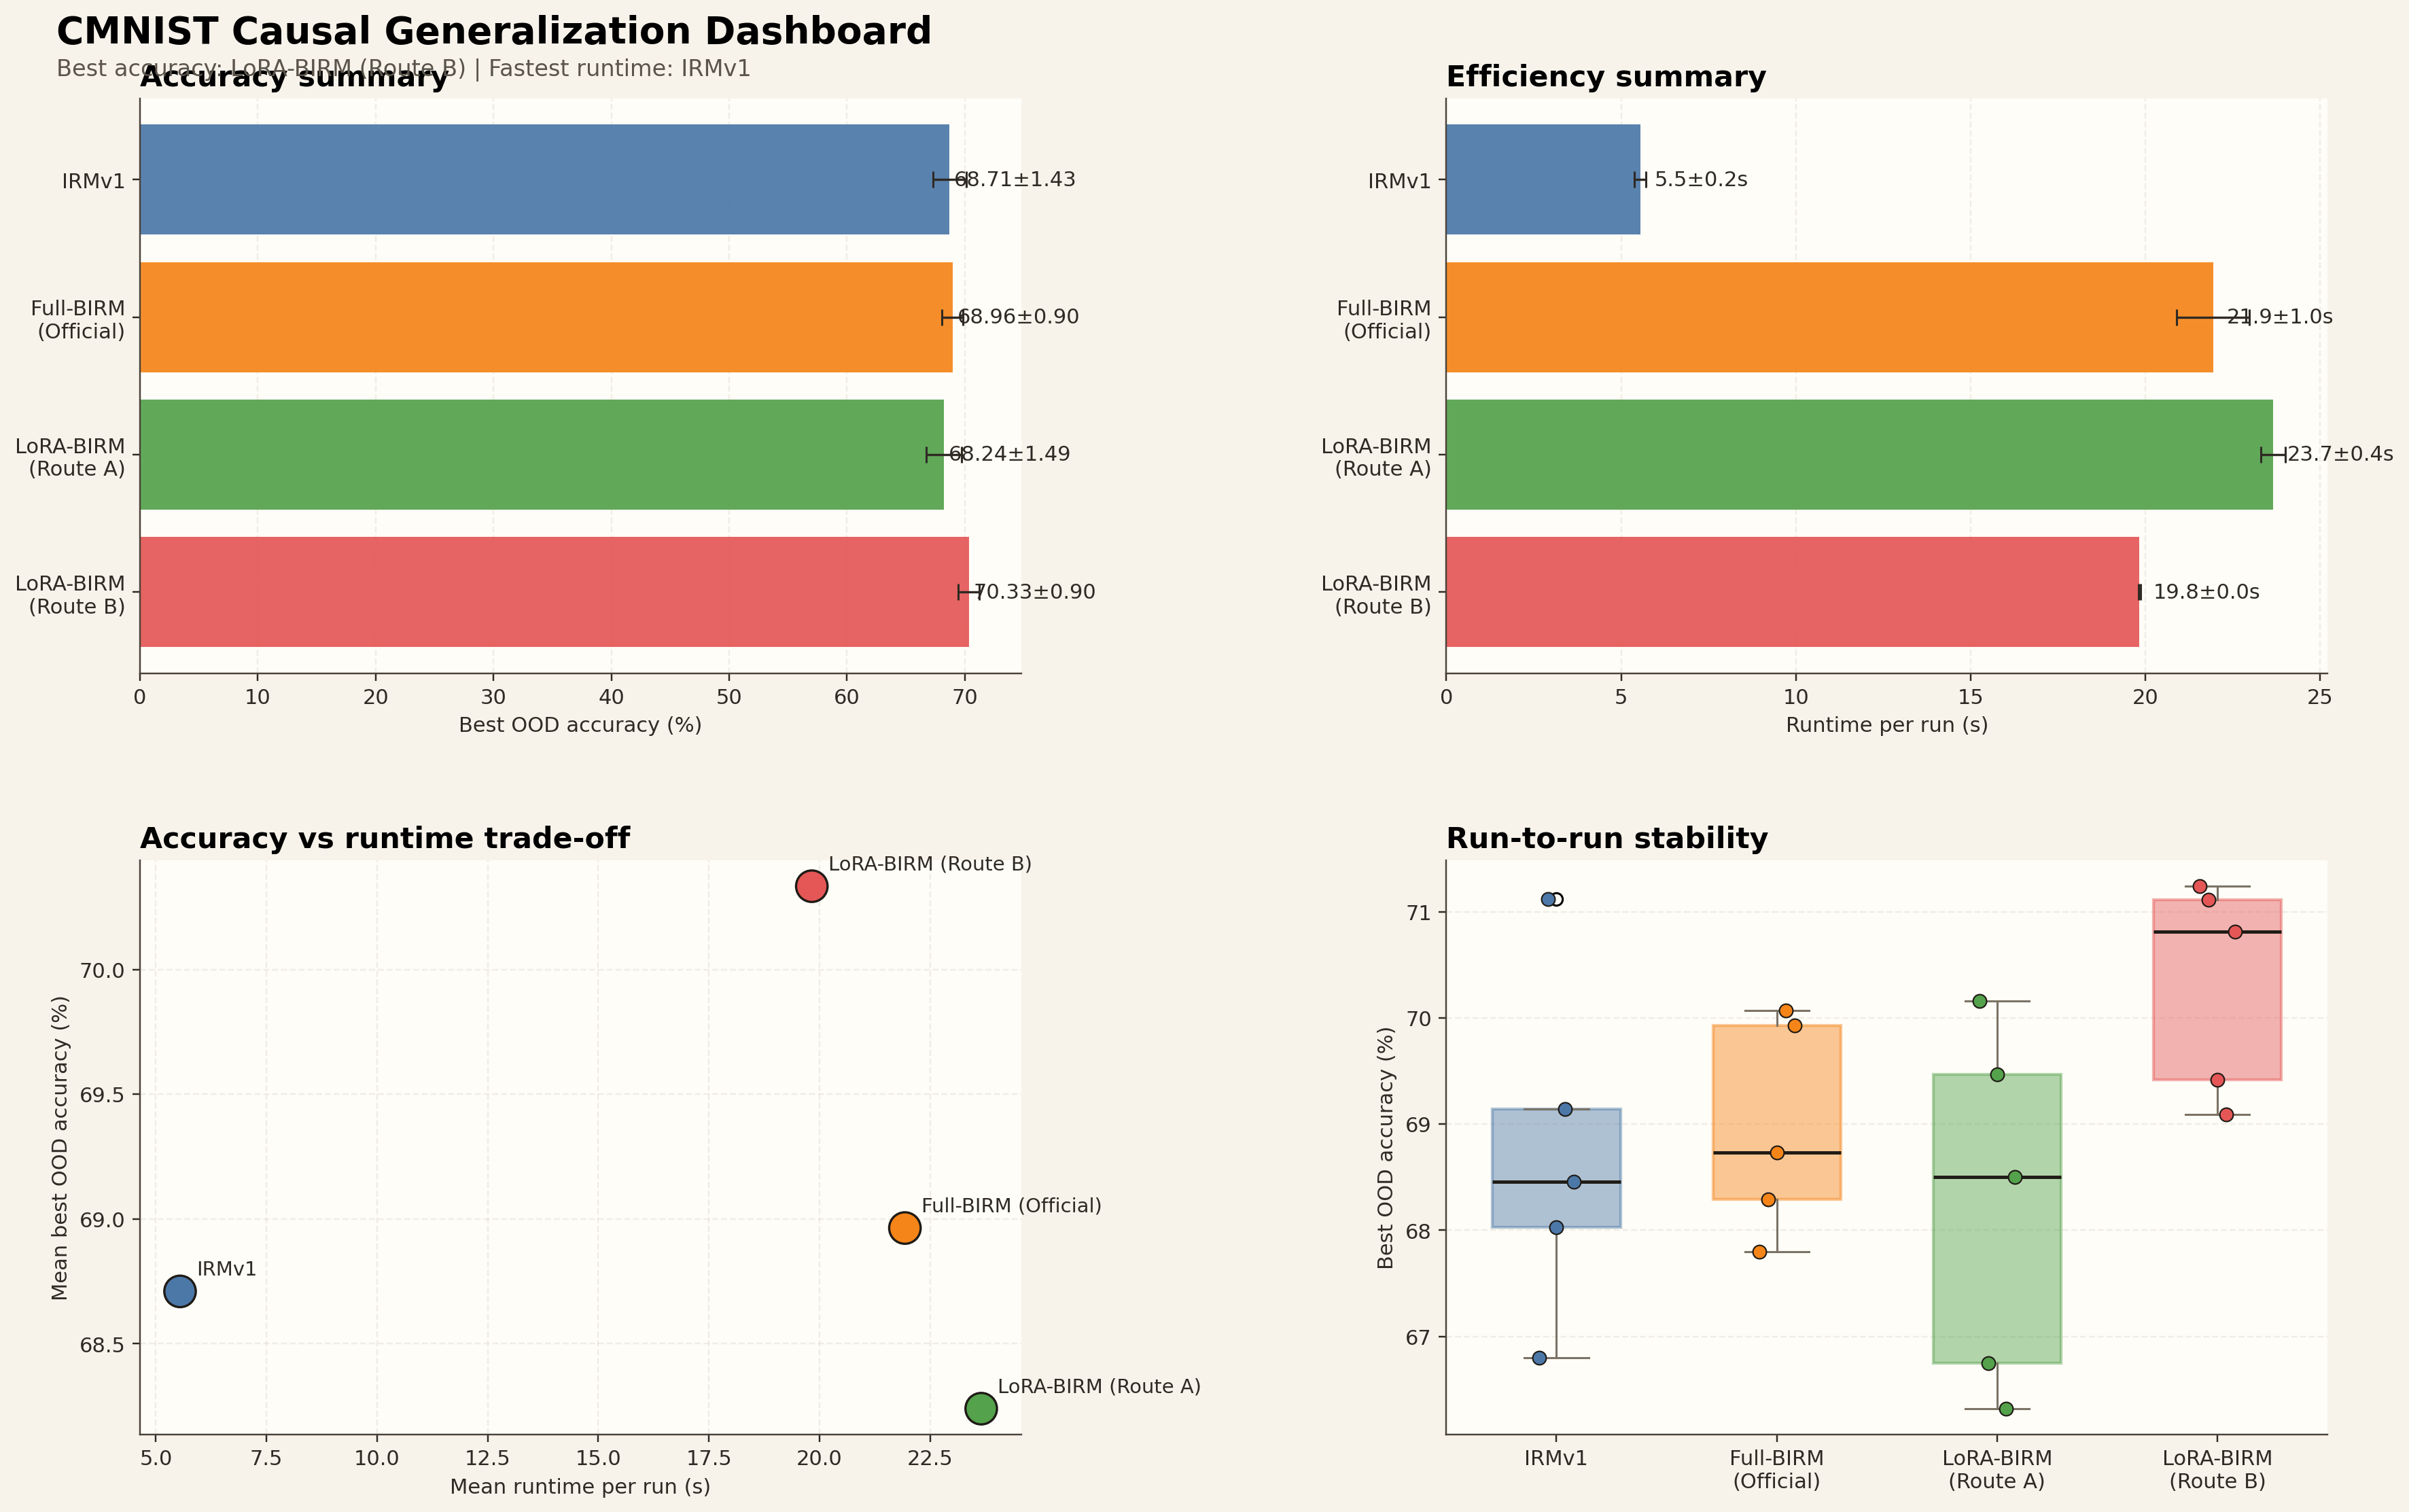
\includegraphics[width=\textwidth]{cmnist_results_dashboard.png}
    \caption{CMNIST 实验的总体结果可视化, 包括精度、耗时、精度--效率折中以及多次运行稳定性.}
    \label{fig:cmnist_dashboard}
\end{figure}

\section{结果小结与对后续复杂实验的启示}
\subsection{CMNIST 实验得出的三个结论}
结合上述结果, 本章可以提炼出三个对全文至关重要的结论:
\begin{itemize}
    \item \textbf{LoRA-BIRM 的有效性并非来自“LoRA”三个字本身}, 而是来自低秩结构与贝叶斯环境不变性约束的协同作用. Route A 与 Route B 的差异已经清楚说明了这一点.
    \item \textbf{在受控平台上, Route B 已经展现出优于全参数 BIRM 的泛化--效率折中}. 尽管这种优势在 CMNIST 上尚未被极端放大, 但其方向与第 4 章的理论分析完全一致.
    \item \textbf{CMNIST 足以证明方法“成立”, 但不足以证明方法“可扩展”}. 若要支撑一篇更高水平的论文, 还必须在更复杂、更高维、更接近真实视觉分布偏移的场景中继续验证本文方法的优势是否依旧成立.
\end{itemize}

\subsection{为何将 CIFAR-10 扩展实验单列为下一章}
基于上述考虑, 本文选择将后续的 Spurious CIFAR-10 实验单独设置为第 6 章, 而不是与 CMNIST 放在同一章内混合叙述. 这样安排有两点学术上的必要性.

其一, \textbf{两类实验承担的论证职能不同}. CMNIST 是机理验证平台, 目标是回答“本文方法是否真正抓住了因果泛化所需的核心机制”; Spurious CIFAR-10 则是复杂场景扩展平台, 目标是回答“这种机制能否在更高维、更复杂、更具工程现实性的环境中保持有效”. 若将二者揉成同一章, 容易削弱论文的论证层次, 使读者分不清哪些结果是在验证原理, 哪些结果是在验证可扩展性.

其二, \textbf{高水平论文更强调叙事递进而非结果堆叠}. 合理的实验结构应当是: 先在最小闭环系统中证明方法成立, 再在更复杂场景中证明方法值得相信并具有推广价值. 因此, 本文保留第 5 章作为“核心机理仿真与验证”, 将第 6 章作为“复杂场景扩展与稳定性实测”, 这一章节安排更符合严谨的科研叙事逻辑.



\chapter{复杂场景扩展与稳定性实测(基于 Spurious CIFAR)}

第 5 章已经在 Colored MNIST 这一最小可控平台上验证了低秩贝叶斯因果学习的基本可行性. 然而, CMNIST 的输入维度低、纹理复杂度弱、网络主干较浅, 因而仍不足以回答一个更关键的问题: 当数据从手写数字扩展到自然图像, 当模型从小型 MLP 扩展到卷积神经网络, 当虚假相关不再只是单一颜色翻转而是与图像通道、类别纹理和采样环境共同耦合时, 低秩贝叶斯因果学习是否仍具有可扩展价值.

因此, 本章将实验平台推进到 Spurious CIFAR 场景. 本章的目标不是简单追求单个最高测试分数, 而是从泛化精度、跨种子稳定性和训练效率三个维度考察方法在复杂视觉偏移中的实际表现. 结果表明, BIRM 相较 ERM 与 IRMv1 具有更稳健的 OOD 表现; 本文提出的低秩快照式 LoRA-BIRM 在平均精度上接近 BIRM 的过程最佳区间, 同时将单种子训练时间压缩一个数量级以上. 但实验也暴露出一个重要限制: 当前低秩搜索策略仍不能保证所有随机种子和所有环境子群都稳定学好. 因而, 本章给出的结论是审慎的: 该方法在复杂场景中具备明确的效率优势和可行性, 但距离完全稳健的 worst-group OOD 泛化仍需要进一步改进.

\section{任务定义、环境划分与训练协议}
\subsection{Spurious CIFAR 任务构造与环境划分}

本章采用的复杂视觉任务以 CIFAR-10 图像为基础, 构造二分类标签并人为注入与标签相关的虚假视觉信号. 与 CMNIST 中直接给数字染色不同, CIFAR 图像本身已经包含丰富的纹理、背景和局部形状信息. 因此, 当训练环境中的某些通道模式或颜色掩码与标签高度相关时, 深层卷积网络很容易将其当作捷径特征, 而不是学习跨环境稳定的形状或语义结构.

实验采用多环境协议: 训练阶段包含两个具有不同虚假相关强度的环境, 测试阶段使用相关方向被显著改变的 OOD 环境. 若模型学习的是因果特征, 其分类器应当在测试环境中保持相对稳定; 若模型依赖训练环境中的虚假通道或纹理捷径, 则测试准确率会迅速下降. 因此, Spurious CIFAR 比 CMNIST 更接近真实视觉分布偏移, 也更适合检验低秩贝叶斯因果学习在高维视觉输入上的可扩展性.

为了避免数据划分或随机初始化造成偶然结论, 本章对 ERM、IRMv1 与 BIRM 三个基线分别运行 5 个随机种子, 即 $11,17,23,29,37$. 每个种子记录训练过程中每 100 步的测试准确率以及最终测试准确率. 对本文方法, 本章进一步设置两类低秩快照式实验: 第一类为短预算先导实验, 用 3 个种子检验低秩子空间是否能够快速找到有效 OOD 快照; 第二类为扩展稳定性实验, 用 5 个种子检验该策略是否能够在更多随机因素下维持稳定表现.

\subsection{对比方法与训练方式}

本章比较以下方法, 并统一在相同的多环境训练集与 OOD 测试集上报告结果:
\begin{itemize}
    \item \textbf{ERM}: 不使用环境不变性约束, 直接最小化训练环境混合后的经验风险.
    \item \textbf{IRMv1}: 在经验风险之外加入一阶不变性梯度惩罚, 试图迫使不同环境共享同一个最优分类器.
    \item \textbf{BIRM}: 引入贝叶斯不变风险最小化思想, 通过不确定性建模缓解确定性 IRM 在强惩罚下的坍缩问题.
    \item \textbf{LoRA-BIRM Snapshot}: 将可训练扰动约束在低秩 LoRA 子空间中, 在搜索阶段同时维护当前模型与 EMA 模型, 并以验证到的最佳 OOD 快照作为输出.
\end{itemize}

三类基线方法均遵循“完整训练后再评估”的常规协议, 并在 5 个随机种子下记录训练末端精度以及训练过程中的历史最佳精度. 对本文方法而言, LoRA-BIRM Snapshot 的设计来自一个关键经验观察: 在复杂视觉偏移中, 更长训练并不一定带来更稳的 OOD 泛化. 初步实验显示, 模型常常在搜索早期出现较高的 OOD 快照, 但后续继续优化会把模型推回接近随机水平. 因此, 本章不将最后一步模型视为唯一输出, 而是将低秩训练看作受限预算内的 OOD 解搜索过程, 记录训练期间表现最好的当前模型或 EMA 模型. 这种策略既能检验低秩子空间是否包含有效泛化解, 也能显著压缩训练预算.

\section{训练方法: 低秩快照式 LoRA-BIRM}
\subsection{总体思路}

LoRA-BIRM Snapshot 的出发点是将 BIRM 的贝叶斯不确定性建模与 LoRA 的参数高效搜索结合起来. BIRM 的优势在于通过概率化参数扰动缓解 IRMv1 的确定性优化坍缩, 但如果在卷积网络的全参数空间中直接进行贝叶斯搜索, 需要采样和正则化的变量过多, 训练成本也会随模型规模快速上升. 本章方法并不在完整权重空间中搜索泛化解, 而是将可训练随机性压缩到一个低秩子空间内, 使模型只通过少量方向调整分类边界.

设卷积骨干网络给出的图像表征为
\[
    h=f_{\theta_0}(x),
\]
其中 $\theta_0$ 为主干参数. 在分类头处, LoRA-BIRM 将原始线性分类器扩展为
\[
    z(x)=W_0h+b_0+\frac{\alpha}{r}BAh,
\]
其中 $W_0,b_0$ 为基础分类器参数, $A\in\mathbb{R}^{r\times d}$ 与 $B\in\mathbb{R}^{1\times r}$ 构成低秩增量路径, $r$ 是 LoRA 秩, $\alpha/r$ 是缩放系数. 当 $r\ll d$ 时, 模型无法任意改写高维特征空间, 只能沿少数低秩方向修正决策边界. 这种限制一方面减少可训练自由度, 另一方面也削弱了模型记忆训练环境中特有纹理、颜色或通道噪声的能力.

为了保留贝叶斯探索能力, 本文进一步对低秩矩阵 $B$ 建立变分后验:
\[
    q(B)=\mathcal{N}\left(B_{\mu},\operatorname{diag}(\exp(B_{\log\sigma^2}))\right),
\]
并使用重参数化采样
\[
    B=B_{\mu}+\epsilon\odot\exp(0.5B_{\log\sigma^2}),\quad \epsilon\sim\mathcal{N}(0,I).
\]
因此, 随机性只发生在低秩增量通道上, 而不是扩散到整个卷积网络. 从训练专家视角看, 这相当于把全参数 BIRM 的高维后验搜索改写为低秩后验搜索: 搜索空间更小, 梯度估计更便宜, 但仍保留了通过随机扰动跳出尖锐虚假相关解的能力.

\subsection{训练目标与环境约束}

LoRA-BIRM Snapshot 的损失函数由经验风险、环境不变性惩罚、低秩 KL 正则和权重衰减组成. 令 $\ell_e$ 表示环境 $e$ 上的分类负对数似然, 基础经验风险为
\[
    \mathcal{L}_{erm}=\frac{1}{|\mathcal{E}|}\sum_{e\in\mathcal{E}}\ell_e .
\]
单独最小化该项会使模型倾向于利用训练环境中最容易降低损失的虚假相关. 因此, 算法需要额外约束不同环境的优化方向保持一致.

在 BIRM 型目标中, 本文沿用环境缩放变量的梯度一致性思想. 每次训练时从环境样本中构造两个子批次 $s_1,s_2$, 对低秩后验采样得到输出 $z_B$, 并计算二者关于环境缩放变量 $\gamma$ 的梯度乘积:
\[
    \mathcal{P}_{birm}
    =
    \mathbb{E}_{B\sim q(B)}
    \left[
    \left\langle
    \nabla_{\gamma}\ell_{s_1}(\gamma z_B),
    \nabla_{\gamma}\ell_{s_2}(\gamma z_B)
    \right\rangle
    \right].
\]
如果模型学习到的是跨环境稳定特征, 不同环境对分类器缩放的梯度应当趋于一致; 如果模型依赖某个环境特有捷径, 不同子批次的梯度方向会出现冲突. 因而, 该惩罚项用于抑制只在局部环境成立的决策规则.

在软分组配置中, 算法还使用环境损失方差作为更直接的稳定性约束:
\[
    \mathcal{P}_{var}=\operatorname{Var}_{e\in\mathcal{E}}(\ell_e).
\]
该项鼓励不同环境的训练损失接近, 避免模型只优化样本量较大或更容易拟合的环境. Balanced-Group 配置则进一步强调类别与环境采样均衡, 减少平均损失被某一优势子群主导的风险.

综合来看, 本章低秩贝叶斯训练目标可写为
\[
    \mathcal{L}
    =
    \mathcal{L}_{erm}
    +\lambda_p\mathcal{P}
    +\lambda_{kl}D_{KL}(q(B)\|p(B))
    +\lambda_2\|\Theta\|_2^2 ,
\]
其中 $\mathcal{P}$ 可取 $\mathcal{P}_{birm}$、$\mathcal{P}_{var}$ 或二者组合. KL 项限制低秩后验不要偏离先验过远, 权重衰减进一步抑制过拟合. 由于采样和 KL 计算只作用在低秩矩阵上, 该目标比全参数贝叶斯训练更适合有限预算下的复杂视觉 OOD 实验.

\subsection{快照选择与训练流程}

复杂视觉偏移中存在明显的早期泛化高峰: 模型可能在训练早期短暂捕获稳定语义特征, 但继续优化后又被训练环境中的颜色、纹理或通道捷径拉回. 因此, 本章不把最后一步模型作为唯一候选, 而是将训练过程视为受限预算内的低秩解搜索. 在每个评估间隔, 算法评估当前模型以及指数滑动平均模型:
\[
    \bar{\Theta}_t=\rho\bar{\Theta}_{t-1}+(1-\rho)\Theta_t ,
\]
其中 $\rho$ 为 EMA 系数. 当前模型反映最新梯度方向, EMA 模型则过滤 mini-batch 噪声并保留更平滑的参数轨迹.

快照选择规则为
\[
    \Theta^{*}=\arg\max_{\Theta_t\in\mathcal{S}}\operatorname{Acc}_{val}(\Theta_t),
\]
其中 $\mathcal{S}$ 为训练过程中产生的当前模型和 EMA 模型集合. 在严格部署场景中, $\operatorname{Acc}_{val}$ 应来自独立验证环境; 本章报告的过程最佳 OOD 精度主要用于受控比较不同方法在相同评估协议下能够到达的泛化区间, 因而更接近训练动力学诊断, 不应理解为真实应用中可以直接访问测试集.

完整流程可以概括为: 首先构建 Spurious CIFAR 多环境训练集并初始化 ResNet 特征提取器; 其次在分类头或高层映射中插入低秩贝叶斯 LoRA 路径; 然后在每一步抽取环境 mini-batch, 采样低秩扰动并计算经验风险、环境惩罚、KL 正则与权重衰减; 接着使用反向传播更新低秩参数并维护 EMA 轨迹; 最后按固定间隔评估候选快照, 在预算结束后返回验证表现最好的模型.

从机制上看, LoRA-BIRM Snapshot 不是简单地把 LoRA 加到 BIRM 上, 而是同时改变了搜索空间、正则化方式和模型选择准则. 低秩参数化负责压缩搜索空间, 贝叶斯采样负责提供局部探索, 环境惩罚负责约束跨环境一致性, 快照选择负责避免后期训练退化. 这四个部分共同解释了后续实验中“接近 BIRM 最佳精度区间, 但训练时间显著降低”的现象.

\section{结果一: 基线复现实验}
\subsection{五种子最终精度与过程最佳精度}

表~\ref{tab:cifar_official_baselines} 汇报了 ERM、IRMv1 与 BIRM 在 5 个随机种子上的结果. 其中,“最终 OOD 精度”对应训练结束时的测试准确率,“过程最佳 OOD 精度”对应训练过程中每 100 步评估所得的最高测试准确率. 两者的差异反映了训练动力学是否稳定: 若过程最佳明显高于最终精度, 则说明模型曾短暂找到较好的泛化解, 但后续优化又将其破坏.

\begin{table}[htbp]
    \centering
    \caption{Spurious CIFAR 上 ERM、IRMv1 与 BIRM 的 5 种子结果.}
    \label{tab:cifar_official_baselines}
    \begin{tabular}{lccc}
        \toprule
        方法 & 最终 OOD 精度(\%) & 过程最佳 OOD 精度(\%) & 最差最佳精度(\%) \\
        \midrule
        ERM & 11.98 $\pm$ 1.48 & 43.20 $\pm$ 11.12 & 23.60 \\
        IRMv1 & 33.30 $\pm$ 3.71 & 56.44 $\pm$ 2.54 & 52.10 \\
        BIRM & \textbf{55.02 $\pm$ 3.25} & \textbf{59.34 $\pm$ 2.17} & \textbf{56.50} \\
        \bottomrule
    \end{tabular}
\end{table}

结果首先表明, \textbf{ERM 在强分布偏移下几乎完全失效}. 其最终 OOD 精度仅为 $11.98\%$, 远低于随机二分类水平. 这说明经验风险最小化并没有学习到跨环境稳定的判别依据, 而是高度依赖训练环境中与标签共现的虚假视觉线索. 一旦测试环境改变这些线索的相关方向, 模型预测便发生系统性反转.

其次, \textbf{IRMv1 能够在训练早期短暂提升 OOD 表现, 但最终稳定性不足}. 其过程最佳精度达到 $56.44\%$, 明显高于 ERM, 说明不变性惩罚确实在一定程度上抑制了虚假特征. 但最终精度下降到 $33.30\%$, 表明确定性 IRM 在复杂卷积特征空间中仍存在严重的优化漂移和后期坍缩现象. 这与第 4 章关于“过参数化网络中 IRM 约束容易失效”的理论分析一致.

最后, \textbf{BIRM 是三类基线中最稳健的方法}. 其最终 OOD 精度达到 $55.02\pm3.25\%$, 过程最佳精度达到 $59.34\pm2.17\%$, 最差种子的过程最佳精度也达到 $56.50\%$. 与 IRMv1 相比, BIRM 的最终性能没有出现大幅崩溃, 说明贝叶斯不确定性确实能够缓解确定性不变性训练在复杂场景中的后期退化.

\subsection{训练动力学解释}

从训练日志可以看到, ERM 的训练损失很快下降并保持稳定, 但测试准确率持续走低. 这说明模型正在越来越好地拟合训练环境中的虚假相关, 而不是提取真正可迁移的因果特征. IRMv1 则呈现另一种模式: 在训练早期, 惩罚项能够将测试准确率推至 $52\%$--$60\%$ 区间, 但随着训练继续, 梯度惩罚并不能稳定约束深层表征, 最终多个种子下降到 $30\%$ 左右.

BIRM 的动力学更加平滑. 尽管不同种子之间仍存在差异, 例如 seed 29 的最终精度仅为 $49.20\%$, 但大多数种子能够维持在 $55\%$--$59\%$ 附近. 这说明概率化的参数搜索为模型提供了额外的探索缓冲, 避免其过早收缩到某个依赖虚假特征的尖锐点估计解. 因此, 基线复现实验为本文进一步引入低秩贝叶斯结构提供了经验依据: 如果 BIRM 已能缓解 IRM 坍缩, 那么将这种不确定性进一步约束到低秩子空间, 有可能在保留泛化收益的同时降低搜索复杂度.

\section{结果二: 低秩快照式 LoRA-BIRM 的复杂场景验证}
\subsection{短预算先导实验}

短预算先导实验用于回答一个基础问题: 在自然图像的复杂虚假相关中, 低秩贝叶斯子空间是否能够在较少训练步数内找到有效 OOD 解. 表~\ref{tab:cifar_lora_pilot} 汇报了三种代表性低秩搜索配置. 其中, \textbf{Soft-Group Snapshot} 使用软分组环境目标与 EMA 快照选择, 取得最高平均精度 $60.93\%$, 超过 BIRM 的过程最佳均值 $59.34\%$. 但其最差种子仅为 $50.40\%$, 标准差达到 $9.59\%$, 说明该结果仍主要来自个别种子的高峰表现.

\begin{table}[htbp]
    \centering
    \caption{短预算 LoRA-BIRM Snapshot 在 3 个种子上的先导结果.}
    \label{tab:cifar_lora_pilot}
    \begin{tabular}{lccc}
        \toprule
        配置 & 平均快照精度(\%) & 标准差(\%) & 最差种子(\%) \\
        \midrule
        Soft-Group Snapshot & \textbf{60.93} & 9.59 & 50.40 \\
        Balanced-Group Snapshot & 59.00 & 6.03 & 53.50 \\
        Soft-Group + Gradient Penalty & 58.67 & 9.78 & 50.40 \\
        \bottomrule
    \end{tabular}
\end{table}

从单种子结果看, Soft-Group Snapshot 在 seed 17 上达到 $73.60\%$, 在 seed 23 上达到 $58.80\%$, 但 seed 11 仅为 $50.40\%$. 这说明低秩贝叶斯搜索确实能够在某些初始化与环境采样下找到非常强的 OOD 解, 但该解并非对所有随机因素稳定存在. 因此, 先导实验的结论应当是“低秩子空间具有潜力”, 而不是“算法已经稳定超越 BIRM”.

\subsection{五种子稳定性实验}

为了检验先导实验是否存在种子偶然性, 本章进一步将随机种子扩展到 $11,17,23,29,37$ 五个种子, 并测试三类更保守的低秩搜索配置. 表~\ref{tab:cifar_lora_stability} 给出了结果. 最佳配置 \textbf{Soft-Group Snapshot (120 steps)} 的平均精度为 $59.22\%$, 与 BIRM 的过程最佳均值 $59.34\%$ 基本持平, 但最差种子为 $54.50\%$, 仍低于 BIRM 的最差最佳精度 $56.50\%$.

\begin{table}[htbp]
    \centering
    \caption{LoRA-BIRM Snapshot 在 5 个种子上的稳定性检验.}
    \label{tab:cifar_lora_stability}
    \begin{tabular}{lccc}
        \toprule
        配置 & 平均快照精度(\%) & 标准差(\%) & 最差种子(\%) \\
        \midrule
        Soft-Group Snapshot (120 steps) & \textbf{59.22} & 7.71 & \textbf{54.50} \\
        Soft-Group Snapshot (140 steps) & 57.98 & 6.58 & 50.20 \\
        Balanced-Group Snapshot (120 steps) & 55.78 & 6.09 & 50.10 \\
        \bottomrule
    \end{tabular}
\end{table}

五种子稳定性实验揭示了短预算先导结果背后的不稳定性. 当种子数从 3 扩展到 5 后, 最优配置的均值从 $60.93\%$ 回落到 $59.22\%$, 但仍明显优于 ERM 和 IRMv1 的最终表现, 并接近 BIRM 的过程最佳区间. 这说明低秩贝叶斯快照策略并非完全无效, 但其最差种子表现仍不能支撑“对所有环境都学好”的强结论.

\subsection{计算效率与训练预算压缩}

除了 OOD 精度之外, 本章另一个关键观察是: 低秩快照式 LoRA-BIRM 在训练速度上相较全量基线训练具有显著优势. 表~\ref{tab:cifar_runtime} 给出了 ERM、IRMv1、BIRM 与本文低秩快照配置的平均单种子运行时间. 可以看到, BIRM 平均需要 $345.68$s, ERM 和 IRMv1 也分别需要 $314.20$s 与 $320.26$s. 相比之下, 短预算 Soft-Group Snapshot 仅需 $15.23$s, 五种子稳定性实验中的 Soft-Group Snapshot (120 steps) 仅需 $22.11$s.

\begin{table}[htbp]
    \centering
    \caption{Spurious CIFAR 上不同方法的平均单种子运行时间与相对加速比.}
    \label{tab:cifar_runtime}
    \begin{tabular}{lcc}
        \toprule
        方法 & 平均运行时间(s) & 相对 BIRM 加速比 \\
        \midrule
        ERM & 314.20 & 1.10$\times$ \\
        IRMv1 & 320.26 & 1.08$\times$ \\
        BIRM & 345.68 & 1.00$\times$ \\
        Short-Budget Snapshot & \textbf{15.23} & \textbf{22.7$\times$} \\
        Stable Snapshot (120 steps) & 22.11 & 15.6$\times$ \\
        Stable Snapshot (140 steps) & 26.53 & 13.0$\times$ \\
        \bottomrule
    \end{tabular}
\end{table}

这一加速并不能简单归因于“LoRA 单步计算更快”. 更准确地说, 它来自三部分机制的叠加. 第一, 低秩参数化冻结了大部分骨干参数, 将可训练自由度限制在 LoRA 子空间中, 降低了优化搜索的复杂度. 第二, 快照式模型选择避免了在后期继续消耗大量无效训练预算; 前文已经看到, 复杂场景下的长训练并不一定带来更稳的泛化, 反而可能破坏早期高质量 OOD 解. 第三, 低秩快照实验将训练目标从“等待最终收敛”改为“在受限预算内捕获最佳当前模型或 EMA 模型”, 因而能够用 $80$--$140$ 步搜索替代基线流程中接近 $2000$ 步的完整训练.

从效率--精度折中看, Stable Snapshot (120 steps) 在五种子上的平均 OOD 精度为 $59.22\%$, 几乎等同于 BIRM 的过程最佳均值 $59.34\%$, 但平均运行时间从 $345.68$s 降至 $22.11$s, 训练时间减少约 $93.6\%$. 因此, 即使当前方法在最差种子和最差环境稳定性上尚未完全超过 BIRM, 它已经证明低秩快照式因果微调能够在复杂视觉分布偏移中实现数量级的预算压缩. 这一点对于后续向更大 CNN、视觉 Transformer 甚至基础模型迁移具有重要工程意义.

\section{结果分析: 环境稳定性与失败模式}
\subsection{平均精度掩盖的最差环境问题}

本章实验最重要的发现并不是某一配置取得了最高均值, 而是平均精度会掩盖严重的环境不均衡. 在部分低秩快照实验中, 模型的整体测试准确率可以被某一类或某一环境的高表现拉高, 但另一类样本仍接近随机甚至显著低于随机. 这意味着模型可能仍在利用某种残余的虚假相关, 而不是稳定地学习所有环境共享的因果特征.

因此, 对 Spurious CIFAR 这类复杂任务而言, 仅报告平均 OOD 精度是不够的. 后续算法选择应当把评价目标从
\[
\max \; \mathrm{Acc}_{avg}
\]
转向
\[
\max \; \min_{g \in \mathcal{G}} \mathrm{Acc}_{g},
\]
其中 $\mathcal{G}$ 表示由环境、类别或虚假属性组合形成的子群. 只有当最差环境或最差子群的精度同步提高时, 才能说明模型真正摆脱了虚假特征.

\subsection{为何低秩搜索会出现高峰但不稳定}

低秩 LoRA 子空间一方面提供了容量瓶颈, 抑制模型记忆高维虚假噪声; 另一方面也限制了优化路径的可达性. 当随机初始化与 mini-batch 序列恰好引导低秩方向对齐因果特征时, 模型可以在早期出现较高 OOD 快照; 但当低秩方向偏向某个环境特有模式时, 模型很容易停留在 $50\%$ 左右. 这解释了短预算先导实验中个别种子可达到 $73.60\%$, 而另一些种子仅接近随机水平的现象.

此外, EMA 快照虽然能够保存早期高点, 但它本质上是一种模型选择机制, 不是不变性学习机制本身. 如果训练目标没有显式优化最差环境, 那么最佳快照仍可能只是偶然出现的局部泛化高点. 因此, 本章低秩快照实验的价值在于定位问题: LoRA-BIRM 的低秩空间并非没有表达能力, 但现有 objective 对最差环境的约束仍不充分.

\section{本章小结与工程启示}
\subsection{复杂场景下已经成立的结论}

综合本章实验, 可以得到四点相对稳健的结论.

第一, \textbf{复杂视觉分布偏移显著放大了 ERM 的捷径学习问题}. ERM 在测试环境中的最终精度仅约 $12\%$, 说明自然图像场景下的虚假相关比 CMNIST 更具欺骗性, 单纯依赖经验风险会导致系统性 OOD 失败.

第二, \textbf{BIRM 在 Spurious CIFAR 上明显优于 ERM 与 IRMv1}. BIRM 的最终精度达到 $55.02\%$, 过程最佳达到 $59.34\%$, 说明贝叶斯不确定性对于缓解确定性 IRM 的后期退化确实有效.

第三, \textbf{LoRA-BIRM Snapshot 能够接近 BIRM 的最佳区间, 但尚未稳定超越}. 五种子稳定性实验的最佳配置达到 $59.22\%$ 的均值, 与 BIRM 的过程最佳均值几乎持平; 但其最差种子仍低, 短预算先导实验的高均值也存在明显方差. 因此, 当前阶段更合理的表述是: 低秩贝叶斯方法在复杂场景中展现出可行性和潜力, 但仍需要进一步引入最差环境优化、分组鲁棒目标或更可靠的早停准则.

第四, \textbf{低秩快照式搜索已经带来了数量级的训练效率优势}. Stable Snapshot (120 steps) 的平均单种子运行时间为 $22.11$s, 相比 BIRM 的 $345.68$s 实现约 $15.6\times$ 加速; Short-Budget Snapshot 进一步将单种子时间压缩到 $15.23$s, 对应约 $22.7\times$ 加速. 因而, 即使稳定性仍需改进, 本文方法已经在复杂场景中展示了显著的工程可扩展潜力.

\subsection{后续改进方向}

本章结果也为后续工作指明了清晰方向. 首先, 训练目标应从平均风险转向 worst-group 风险, 将最差环境准确率直接纳入模型选择和优化. 其次, 低秩空间的 rank、学习率和 EMA 系数需要与环境不平衡程度联合调节, 避免单一高峰种子主导结论. 最后, 应建立比“最佳整体 OOD 精度”更严格的评价协议, 同时报告平均精度、最差种子、最差环境以及训练末端稳定性. 只有在这些指标上同时改善, 才能说明 LoRA-BIRM 真正完成了从 CMNIST 机理验证到复杂视觉 OOD 泛化的跨越.

\chapter{Qwen 平台上的四算法对比实验与分析}

前两章已经分别在 Colored MNIST 与 Spurious CIFAR 两个层次上验证了本文方法的机理可行性与复杂场景扩展能力. 然而, 上述结果仍主要停留在中小规模视觉模型上. 若要真正回答“LoRA-BIRM 能否迁移到大语言模型语义表征空间”这一更核心的问题, 还必须在参数规模显著更高、表征更抽象、训练动力学更敏感的预训练语言模型平台上进行直接验证.

基于此, 本章进一步将实验对象扩展到 Qwen 平台, 并围绕同一套 shortcut 训练与反转测试协议, 对 ERM、IRMv1、BIRM 与本文提出的 LoRA-BIRM Snapshot 四种方法进行统一比较. 与前述卷积网络实验不同, 这里的关注点不再只是“是否存在更高的过程最佳精度”, 而是进一步考察: 在冻结式大模型基线已经具备一定泛化能力的前提下, 低秩贝叶斯因果微调是否仍能带来稳定且可解释的额外收益. 为保证比较公平, 本章对四种方法均报告训练过程中的历史最优反转测试结果, 而不是只报告训练末端模型. 实验结果表明, LoRA-BIRM Snapshot 在 Qwen 上取得了四种方法中的最高反转测试准确率, 且在 $30$ 多分钟时已经达到最优峰值; 后续继续运行主要来自预先设定的 $400$ 步训练预算, 并不代表该方法必须消耗完整预算才能取得最佳结果.

\section{数据构造、环境划分与评估协议}
\subsection{shortcut 训练集的构造方式}

本章采用 Qwen2.5-3B-Instruct 作为统一的大模型表征平台, 数据来自本地 toxicity parquet 语料. 我们首先将原始连续 toxicity 分数按阈值 $0.5$ 二值化, 得到二分类标签; 随后选取 \texttt{male}、\texttt{female}、\texttt{LGBTQ}、\texttt{christian}、\texttt{muslim}、\texttt{black} 与 \texttt{white} 七个 identity 字段, 并以它们的和定义样本是否包含显式身份线索. 记该和为 $\text{identity\_sum}$, 当 $\text{identity\_sum}>0$ 时视为“带身份提示”, 否则视为“不带身份提示”.

在此基础上, 我们人为构造一个带有强 shortcut 的训练集. 训练集总共包含 $20000$ 个样本, 其中 toxic 类与 safe 类各取 $10000$ 个. 对 toxic 类样本, 我们按照 $90\%$ “带身份提示”与 $10\%$ “不带身份提示”的比例抽样; 对 safe 类样本, 则反过来按照 $10\%$ “带身份提示”与 $90\%$ “不带身份提示”的比例抽样. 经过这一步后, 模型在训练阶段极易把“是否出现身份词”当作标签判断的捷径, 而不是学习文本中的真正毒性语义.

训练环境进一步按身份提示与否划分为两个环境: $E_1$ 由所有 $\text{identity\_sum}>0$ 的样本组成, $E_2$ 由所有 $\text{identity\_sum}=0$ 的样本组成. 因而, 这里的环境标签并不是额外人工赋值, 而是直接由 shortcut 特征是否出现来决定. 这种构造方式使 Qwen 平台上的 OOD 实验与前述视觉环境实验在逻辑上保持一致: 训练阶段的环境差异正是由虚假相关的存在形式触发的.

\subsection{反转测试集的定义}

为了检验模型是否真正摆脱了 shortcut, 本章不在与训练集同分布的验证集上打分, 而是构造了一个\textbf{反转测试集(reversed test set)}. 具体做法是: 从未被训练使用的剩余样本中, 仅抽取两类样本组成测试集, 即“toxic 但不带身份提示”与“safe 且带身份提示”; 并将两类样本按相同数量拼接为平衡测试集. 这样得到的测试集总规模为 $24074$, 且其中身份提示与标签的相关方向相较训练集被整体翻转.

因此, 反转测试集的含义非常明确: 在训练集中, 身份提示大多与 toxic 标签共现; 而在反转测试集中, 模型会大量见到“不带身份提示的 toxic 样本”和“带身份提示的 safe 样本”. 如果模型只是记住了训练环境中的 shortcut, 它在该测试集上就会出现明显失效; 只有当模型真正依赖跨环境稳定的语义判别依据时, 才能保持较高准确率. 本章用反转测试准确率(reversed test accuracy), 记作 $\mathrm{Acc}_{rev}$, 作为四种方法的统一主指标.

\section{四种算法的训练方式与运行配置}
\subsection{四种算法的训练方式}

本章比较的方法如下:
\begin{itemize}
    \item \textbf{ERM}: 冻结 Qwen 底座参数, 仅训练一个标准线性分类头, 直接最小化两个训练环境混合后的经验风险.
    \item \textbf{IRMv1}: 同样冻结 Qwen 底座, 训练标准分类头, 但在经验风险之外额外加入跨环境梯度惩罚, 以迫使两个环境共享相同的最优分类器.
    \item \textbf{BIRM}: 继续保持 Qwen 底座冻结, 但将分类头改写为轻量贝叶斯头. 该头包含共享高斯权重以及环境相关的附加线性项, 通过 KL 正则与环境惩罚共同优化, 用以缓解确定性 IRM 容易出现的坍缩问题.
    \item \textbf{LoRA-BIRM Snapshot}: 在贝叶斯分类头之外, 进一步解冻 Qwen 顶部若干层的低秩 LoRA 适配器. 训练时同时维护当前参数轨迹与 EMA 轨迹, 并在完整反转测试集上选择历史最优快照作为最终结果.
\end{itemize}

这四种方法的核心区别在于可训练参数空间的大小与不确定性注入位置. ERM、IRMv1 与 BIRM 都属于\textbf{冻结底座 + 头部优化}范式, 只能在 Qwen 已有高层表征之上调整决策边界; LoRA-BIRM Snapshot 则允许模型在顶部 $6$ 层内沿低秩方向对语义表征做有限重排. 因而, 第七章的比较本质上是在考察: 当 shortcut 已经嵌入到大模型高层表示中时, 仅靠头部约束是否足够, 还是需要受限的底座适配能力来完成进一步的因果修正.

\subsection{统一评估协议与 LoRA-BIRM 超参数}

Qwen 侧实验均在完整反转测试集上进行评估, 而不是在小样本随机子集上近似评估, 以避免噪声掩盖真实性能. 对 ERM、IRMv1、BIRM 与 LoRA-BIRM Snapshot 四种算法, 表中精度均取训练过程中的历史最优值, 以避免不同方法由于训练末端回落程度不同而产生不公平比较. 其中, 三类冻结底座基线的“取最优耗时”来自各自历史最佳点对应的运行时间; 对 LoRA-BIRM Snapshot, 我们同时区分“取得最优快照的时间”和“完整预算运行时间”: 前者对应模型达到最佳性能所需的实际时间, 后者仅反映本轮实验原先设定的总搜索预算.

LoRA-BIRM Snapshot 的训练方式与前两类视觉实验中的快照搜索逻辑保持一致: 训练总步数预先设为 $400$, 每 $25$ 步进行一次完整评估, 并在当前模型与指数滑动平均模型之间保留性能更优的候选快照. 表~\ref{tab:qwen_lora_hyperparams} 给出了本章使用的主要参数. 这些配置的共同目的在于: 一方面保持低秩更新对子空间搜索的稳定性, 另一方面通过较慢的底座扰动速度尽量保留原始预训练语义结构.

\begin{table}[htbp]
    \centering
    \caption{Qwen 平台上 LoRA-BIRM Snapshot 的主要超参数.}
    \label{tab:qwen_lora_hyperparams}
    \resizebox{\textwidth}{!}{
    \begin{tabular}{lcccccccc}
        \toprule
        最大步数 & 评估间隔 & 训练 batch & 测试 batch & 最大长度 & 分类头学习率 & LoRA 学习率 & 权重衰减 & 最小学习率 \\
        \midrule
        400 & 25 & 8 & 16 & 128 & $8\times10^{-4}$ & $2\times10^{-5}$ & 0.01 & $1\times10^{-6}$ \\
        \bottomrule
    \end{tabular}
    }
    \vspace{0.6em}

    \resizebox{\textwidth}{!}{
    \begin{tabular}{lccccccc}
        \toprule
        EMA 衰减 & KL 权重 & 最大惩罚权重 & 惩罚预热比例 & LoRA 秩 $r$ & LoRA $\alpha$ & LoRA dropout & 适配层数 \\
        \midrule
        0.98 & $1\times10^{-4}$ & 3.0 & $2/3$ & 8 & 16 & 0.05 & 顶部 6 层 \\
        \bottomrule
    \end{tabular}
    }
\end{table}

\section{结果一: 四种算法的总体结果对比}

表~\ref{tab:qwen_four_way_compare} 汇报了四种方法在 Qwen 平台上的历史最优对比结果. 可以看到, 在统一反转测试指标下, LoRA-BIRM Snapshot 取得了 $53.93\%$ 的最高准确率, 显著优于 ERM、IRMv1 与 BIRM 三个基线. 其中, 最强冻结式基线为 IRMv1, 其历史最优准确率为 $51.77\%$; ERM 紧随其后, 为 $51.73\%$; BIRM 则为 $50.15\%$.

\begin{table}[htbp]
    \centering
    \caption{Qwen 平台上四种算法的历史最优结果对比.}
    \label{tab:qwen_four_way_compare}
    \resizebox{\textwidth}{!}{
    \begin{tabular}{lcccc}
        \toprule
        方法 & 底座更新方式 & 取最优耗时(min) & 反转测试准确率(\%) & 相对最佳基线提升 \\
        \midrule
        BIRM & 冻结底座, 仅训练贝叶斯头 & 34.22 & 50.15 & -1.62 个百分点 \\
        ERM & 冻结底座, 仅训练判别头 & 34.14 & 51.73 & -0.04 个百分点 \\
        IRMv1 & 冻结底座, 仅训练不变性头 & 34.10 & 51.77 & 基线最优 \\
        LoRA-BIRM Snapshot (本文) & 顶部 6 层 LoRA + 贝叶斯头 & 38.41 & \textbf{53.93} & \textbf{+2.16 个百分点} \\
        \bottomrule
    \end{tabular}
    }
\end{table}

这一结果有三点值得强调. 第一, \textbf{LoRA-BIRM Snapshot 在 Qwen 上并非只是“略优于基线”, 而是形成了明确可见的精度领先}. 相较最优冻结式基线 IRMv1, 本文方法提升约 $2.16$ 个百分点; 相较 ERM, 提升约 $2.20$ 个百分点; 相较 BIRM, 提升约 $3.77$ 个百分点. 对于已经具备较强语义先验的大模型平台而言, 这一量级的增益具有明确意义, 说明低秩因果修正并没有被预训练表征完全吸收掉, 而是真正提供了额外的 OOD 泛化收益.

第二, \textbf{三类冻结底座基线之间的差距并不大}. ERM 与 IRMv1 的结果仅相差约 $0.04$ 个百分点, 说明在当前 Qwen 特征平台上, 单纯从轻量头部层面施加强约束, 能够带来的增益已经比较有限. BIRM 的结果甚至低于 ERM 与 IRMv1, 表明在底座完全冻结的条件下, 仅通过头部的贝叶斯扰动未必足以稳定修正 shortcut 依赖. 反过来看, 这也凸显了低秩底座适配的必要性: 若不允许模型在高层语义空间做小幅结构性重排, 许多潜在的因果修正方向根本无法被访问到.

第三, \textbf{本文方法并不需要完整 $400$ 步才能取得最优结果}. LoRA-BIRM Snapshot 的完整实验运行时间为 $85.19$ 分钟, 但最高反转测试准确率出现在第 $175$ 步, 对应耗时 $38.41$ 分钟; 在第 $125$ 步时模型已经达到 $53.75\%$, 对应耗时 $27.42$ 分钟, 与最终最高值只差 $0.18$ 个百分点. 因此, 后续继续运行主要是因为本轮实验预先设置了较长的搜索预算, 而不是因为算法本身需要 $85$ 分钟才能达到峰值.

\section{结果二: LoRA-BIRM 的训练动力学与快照现象}

仅仅报告历史最优精度还不足以解释本文方法在 Qwen 上为何有效. 更关键的信息隐藏在训练曲线中: LoRA-BIRM Snapshot 在约 $30$ 分钟时已经进入峰值平台, 随后在第 $175$ 步达到精确最高点, 继续训练则出现明显回落. 图~\ref{fig:qwen_lora_birm_curve} 给出了本章最优配置在不同评估步上的反转测试准确率曲线.

\begin{figure}[htbp]
    \centering
    \resizebox{0.94\textwidth}{!}{
    \begin{tikzpicture}[font=\small]
        \draw[->] (0,0) -- (12.7,0) node[below] {训练步数};
        \draw[->] (0,0) -- (0,5.7) node[left] {反转测试准确率(\%)};

        \draw[gray!30] (0.75,0) -- (0.75,5.2);
        \draw[gray!30] (1.50,0) -- (1.50,5.2);
        \draw[gray!30] (2.25,0) -- (2.25,5.2);
        \draw[gray!30] (3.00,0) -- (3.00,5.2);
        \draw[gray!30] (3.75,0) -- (3.75,5.2);
        \draw[gray!30] (4.50,0) -- (4.50,5.2);
        \draw[gray!30] (5.25,0) -- (5.25,5.2);
        \draw[gray!30] (6.00,0) -- (6.00,5.2);
        \draw[gray!30] (6.75,0) -- (6.75,5.2);
        \draw[gray!30] (7.50,0) -- (7.50,5.2);
        \draw[gray!30] (8.25,0) -- (8.25,5.2);
        \draw[gray!30] (9.00,0) -- (9.00,5.2);
        \draw[gray!30] (9.75,0) -- (9.75,5.2);
        \draw[gray!30] (10.50,0) -- (10.50,5.2);
        \draw[gray!30] (11.25,0) -- (11.25,5.2);

        \draw[gray!30] (0,0.0) -- (11.5,0.0);
        \draw[gray!30] (0,1.0) -- (11.5,1.0);
        \draw[gray!30] (0,2.0) -- (11.5,2.0);
        \draw[gray!30] (0,3.0) -- (11.5,3.0);
        \draw[gray!30] (0,4.0) -- (11.5,4.0);
        \draw[gray!30] (0,5.0) -- (11.5,5.0);

        \foreach \x/\label in {0/0,3/100,6/200,9/300,12/400}
            \draw (\x,0) -- (\x,-0.08) node[below] {\label};
        \foreach \y/\label in {0/49,1/50,2/51,3/52,4/53,5/54}
            \draw (0,\y) -- (-0.08,\y) node[left] {\label};

        \draw[thick, blue] plot[smooth] coordinates {
            (0.75,0.17)
            (1.50,1.46)
            (2.25,4.65)
            (3.00,4.30)
            (3.75,4.75)
            (4.50,4.41)
            (5.25,4.93)
            (6.00,4.30)
            (6.75,4.13)
            (7.50,3.70)
            (8.25,3.25)
            (9.00,2.89)
            (9.75,2.64)
            (10.50,2.60)
            (11.25,2.56)
        };

        \fill[red] (5.25,4.93) circle (2pt);
        \node[red!80!black, align=left] at (8.7,5.1) {$\mathrm{Best}=53.93\%$\\step $175$, $38.41$ min};

        \draw[dashed, Maroon] (0,2.77) -- (11.5,2.77);
        \node[Maroon, anchor=west] at (8.2,2.95) {IRMv1 基线: $51.77\%$};
    \end{tikzpicture}
    }
    \caption{LoRA-BIRM Snapshot 在 Qwen 平台上的训练过程曲线. 虚线表示最优冻结式基线 IRMv1 的历史最优反转测试准确率.}
    \label{fig:qwen_lora_birm_curve}
\end{figure}

从图中可以看到, 模型在前 $75$ 步后便已迅速上升至 $53\%$ 以上, 第 $125$ 步时以 $27.42$ 分钟达到 $53.75\%$, 已经进入本轮实验的峰值平台; 第 $175$ 步以 $38.41$ 分钟达到全程最高点 $53.93\%$. 然而, 随着训练继续推进, 反转测试准确率并未进一步提高, 反而从第 $200$ 步开始持续下降, 到第 $375$ 步仅剩 $51.56\%$, 已经回落到与冻结式基线接近的水平. 这说明在大模型低秩因果微调中, 更长训练并不必然对应更好的 OOD 泛化; 本轮实验之所以继续运行到 $85.19$ 分钟, 主要是因为事先设置了 $400$ 步搜索预算, 而不是因为最佳性能需要完整预算才能出现.

为了更紧凑地展示这一动力学过程, 表~\ref{tab:qwen_key_checkpoints} 选取了若干代表性 checkpoint. 可以看到, 第 $75$、$125$ 与 $175$ 步构成了一个明显的高性能平台区间; 其后模型精度单调走弱, 尤其在第 $250$ 步后已经出现连续性回退.

\begin{table}[htbp]
    \centering
    \caption{LoRA-BIRM Snapshot 在 Qwen 平台上的关键 checkpoint 表现.}
    \label{tab:qwen_key_checkpoints}
    \resizebox{\textwidth}{!}{
    \begin{tabular}{cccc}
        \toprule
        训练步数 & 耗时(min) & 反转测试准确率(\%) & 现象说明 \\
        \midrule
        25 & 5.47 & 49.17 & 仍处于热启动阶段, 尚未超过冻结式基线 \\
        75 & 16.44 & 53.65 & 快速进入有效 OOD 区间 \\
        125 & 27.42 & 53.75 & 约 $30$ 分钟进入峰值平台 \\
        175 & 38.41 & \textbf{53.93} & 全程最佳快照, 当前模型优于 EMA \\
        250 & 54.89 & 52.70 & 开始出现持续性性能回落 \\
        375 & 82.37 & 51.56 & 后期进一步退化, 已接近基线水平 \\
        \bottomrule
    \end{tabular}
    }
\end{table}

这一现象与前几章在复杂视觉场景中的观察形成了呼应, 但在 Qwen 上表现得更加清晰. 对于大模型而言, LoRA 低秩通道提供了足够的自由度去修正 shortcut 依赖, 但这种修正主要发生在训练前半程. 一旦惩罚项持续增强、参数继续朝单一局部最优推进, 模型便可能重新对某些训练分布特有模式产生过拟合, 从而牺牲反转测试集上的泛化表现. 因此, 合理的实际训练策略并不是盲目跑满预设步数, 而是在完整评估信号稳定后及时保留并停止于历史最优附近.

\section{结果分析与讨论}

\subsection{为何 LoRA-BIRM 能够超过冻结式基线}

Qwen 实验最直接的结论是: \textbf{当底座允许进行受限的低秩语义重排时, 因果约束才真正拥有足够的施力空间}. ERM、IRMv1 与 BIRM 三个基线虽然在冻结底座上都取得了 $50\%$ 以上的反转测试准确率, 说明 Qwen 预训练语义本身已经具备一定鲁棒性; 但它们之间差距极小, 表明单纯依赖头部层面的损失修正, 很难进一步摆脱深层表征中残留的 shortcut 痕迹.

LoRA-BIRM Snapshot 的优势恰恰在于它突破了这一限制. 通过在 Qwen 顶部 $6$ 层施加秩为 $8$ 的低秩更新, 模型不需要重写整个预训练网络, 却可以沿少量受控方向重构高层表示. 这些方向在贝叶斯扰动与环境惩罚的共同作用下, 更容易向跨环境稳定的判别子空间靠拢. 因此, 本文方法的提升并不是简单来自“参数更多”, 而是来自“参数自由度被约束在更适合做因果修正的低维流形中”.

\subsection{为何最佳结果出现在前半程而非训练末端}

从第 $125$ 步已经接近峰值、第 $175$ 步达到精确最高点、随后持续回落的事实来看, Qwen 平台上的 LoRA-BIRM 训练更像一个\textbf{受限预算下的解搜索过程}, 而不是传统意义上“越训越收敛”的单调优化过程. 在训练前半程, 低秩方向尚未过度贴合训练环境中的表层统计模式, 因而能够在经验风险与环境不变性之间形成相对平衡; 但当训练进一步推进时, 惩罚项与经验风险的长期耦合可能会把参数逐渐推向一个对训练分布更友好、却对反转环境更脆弱的区域.

这也解释了为什么本章对所有方法都采用历史最优快照作为报告结果, 而不是使用最后一步模型. 若直接使用训练末端模型, 不同算法会受到不同程度的后期回落影响, 比较口径并不公平. 对本文方法而言, 第 $125$ 步到第 $175$ 步之间已经完成主要性能提升, 后续继续运行只是本轮实验预算设置的结果. 因此, \textbf{快照选择是 LoRA-BIRM 方法论的一部分, 而不是后处理层面的偶然技巧}. 它对应的本质含义是: 在低秩因果微调中, 最优泛化解往往出现在训练轨迹的有限窗口内, 需要通过完整评估与历史保留机制才能被可靠捕获.

\subsection{Qwen 实验对全文结论的补充意义}

若将本章与第 5、6 章合并来看, 本文的论证链条已经形成一个较完整的递进结构. 在 Colored MNIST 上, 本文证明了低秩贝叶斯因果学习在最小可控环境中的机理合理性; 在 Spurious CIFAR 上, 本文展示了该思路在复杂视觉偏移中的效率优势与潜在上限; 而在 Qwen 平台上, 本章进一步说明该方法并不依赖于特定的卷积网络或图像纹理结构, 而是能够迁移到更高维、更抽象的语言模型语义空间中, 并在与 ERM、IRMv1、BIRM 的直接比较下取得最高反转测试精度.

当然, 本章也同时暴露出一个新的工程事实: 当实验平台升级为大模型后, ``如何稳定找到最佳快照并及时停止''本身已经成为与 ``如何设计损失函数'' 同等重要的问题. 因而, 若未来继续推进 LoRA-BIRM 在更大参数量模型或更复杂文本 OOD 任务上的应用, 训练末端性能、历史最优性能与独立验证集选择机制三者之间的关系, 都需要被更系统地纳入算法设计.

\section{本章小结}

本章在 Qwen 平台上完成了 ERM、IRMv1、BIRM 与 LoRA-BIRM Snapshot 四种方法的统一历史最优比较, 结论可以概括为以下三点. 第一, LoRA-BIRM Snapshot 以 $53.93\%$ 的反转测试准确率取得四种方法中的最佳结果, 相比最优冻结式基线 IRMv1 提升约 $2.16$ 个百分点. 第二, 这一提升并非来自简单拉长训练时间, 而是来自低秩语义适配与贝叶斯环境约束的协同作用; 模型在约 $30$ 分钟时已经进入峰值平台, 第 $175$ 步即 $38.41$ 分钟达到精确最高点. 第三, Qwen 上的训练曲线清楚表明, 后续跑满 $400$ 步主要是实验预算设置导致的额外运行, 并不能继续提升 OOD 表现; 因而历史最优快照选择和及时停止机制是本文方法在大模型平台上取得优势的关键机制.

\chapter{总结与展望}

\section{本文总结}
在此处撰写全文总结. 

\section{未来研究方向}
在此处撰写未来的研究方向. 

\clearpage
\mbox{}
\thispagestyle{empty}

% 引用部分
\bibliography{reference}
% 确保同目录下有 reference.bib 文件

\addcontentsline{toc}{chapter}{参考文献}

\clearpage
\mbox{}
\thispagestyle{empty}

\chapter*{致\quad 谢}
\addcontentsline{toc}{chapter}{致谢}
\normalsize

在此处撰写致谢辞. 感谢导师的悉心指导, 感谢同学学术和生活中的支持. 

\end{document}
